\subsection{Identity and colours}
\hspace{\parindent}The official name of the app is 'Polaris'. The app identity is an astronaut, with the idea of a user acting as an astronaut, which has an overview of the planet Earth and can just pick a place and travel wherever. This feature is also presented in one of the screens in the app, as user searches for already existing trips by searching the globe.

\begin{figure}[!htb]
\centering

\includegraphics[width=0.4\textwidth]{../Images/PolarisIcon.png}
\caption{\label{fig:dbapiuser}\textbf{'Polaris' icon featuring an astronaut on a blue background}}
\end{figure} 

The main colours used for the app are two slightly different blues. Primary blue has the RBG value of \#0083FF while secondary blue has the RBG value of \#0460D9. They are used interchangeably throughout the app.
\begin{figure}[!htb]
\centering
\begin{minipage}{.45\textwidth}
\centering
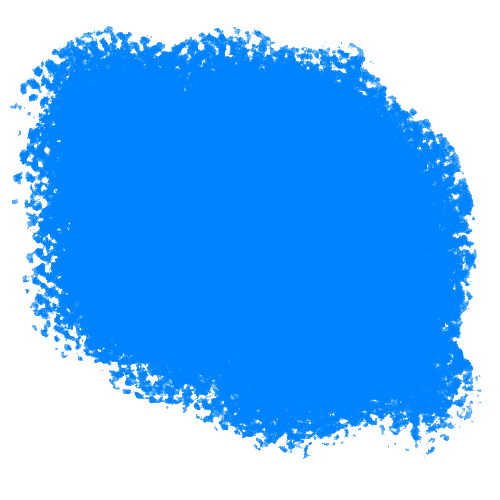
\includegraphics[width=.5\textwidth]{../Images/UI/primaryColor.png}
\caption{\label{fig:dbapiuser}\textbf{Primary color \#0083FF}}
\end{minipage} 
\begin{minipage}{.45\textwidth}
\centering
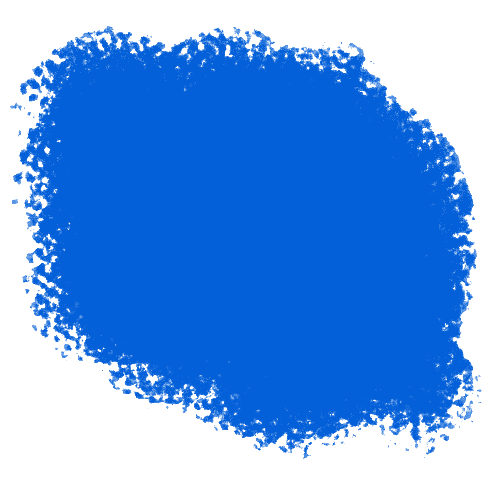
\includegraphics[width=.5\textwidth]{../Images/UI/secondaryColor.png}
\caption{\label{fig:dbapiuser}\textbf{Secondary color \#0460D9}}
\end{minipage}
\end{figure} 

As app features both light and dark mode, there are also colour palettes used for those instances. The same primary and secondary colours are used for accents, but for backgrounds and texts, the colours presented in the following two figures are used. 

\begin{figure}[!htb]
\centering
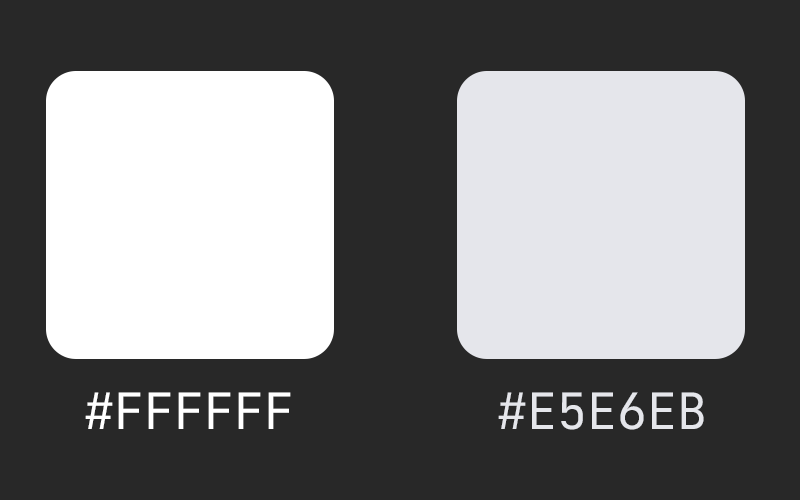
\includegraphics[width=0.7\textwidth]{../Images/UI/BackgroundLight.png}
\caption{\label{fig:dbapiuser}\textbf{Background colours for light theme}}
\end{figure} 

\begin{figure}[!htb]
\centering
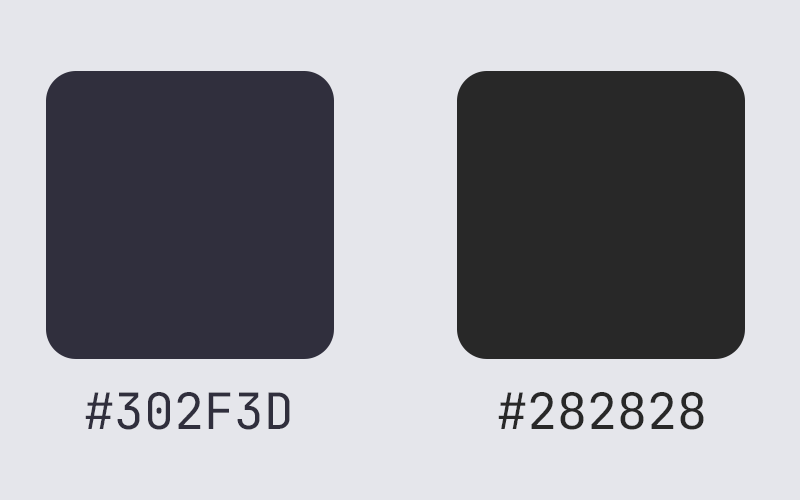
\includegraphics[width=0.7\textwidth]{../Images/UI/BackgroundDark.png}
\caption{\label{fig:dbapiuser}\textbf{Background colours for dark theme}}
\end{figure} 
\newpage

\subsection{User interface design}

\hspace{\parindent}This section features the main design choices of the entire UI of the app, which includes navigation bars, menus, buttons, and other choices. It will not go into too much detail about every component, as all of the screens will be shown with a short comment about it. \\ \\
The main part of the app is divided into four major components, with additional screens available for other functionalities, such as adding and editing destinations and trips. At the bottom of the app there is a navigation bar that leads the user to all of the main screens. Additionally, users can navigate to the settings/account screen either by pressing the 'Polaris' icon in the upper right corner of the screen, or by pressing the last icon in the bottom navigation bar. Right above the navigation bar, a search bar is located which allows the users to search for their previously saved trips.\\ \\
As previously mentioned, the app features both light and dark themes. The following figures present the same screens for both of the themes.\\

\subsection{Login screen}
\begin{figure}[!htb]
\centering
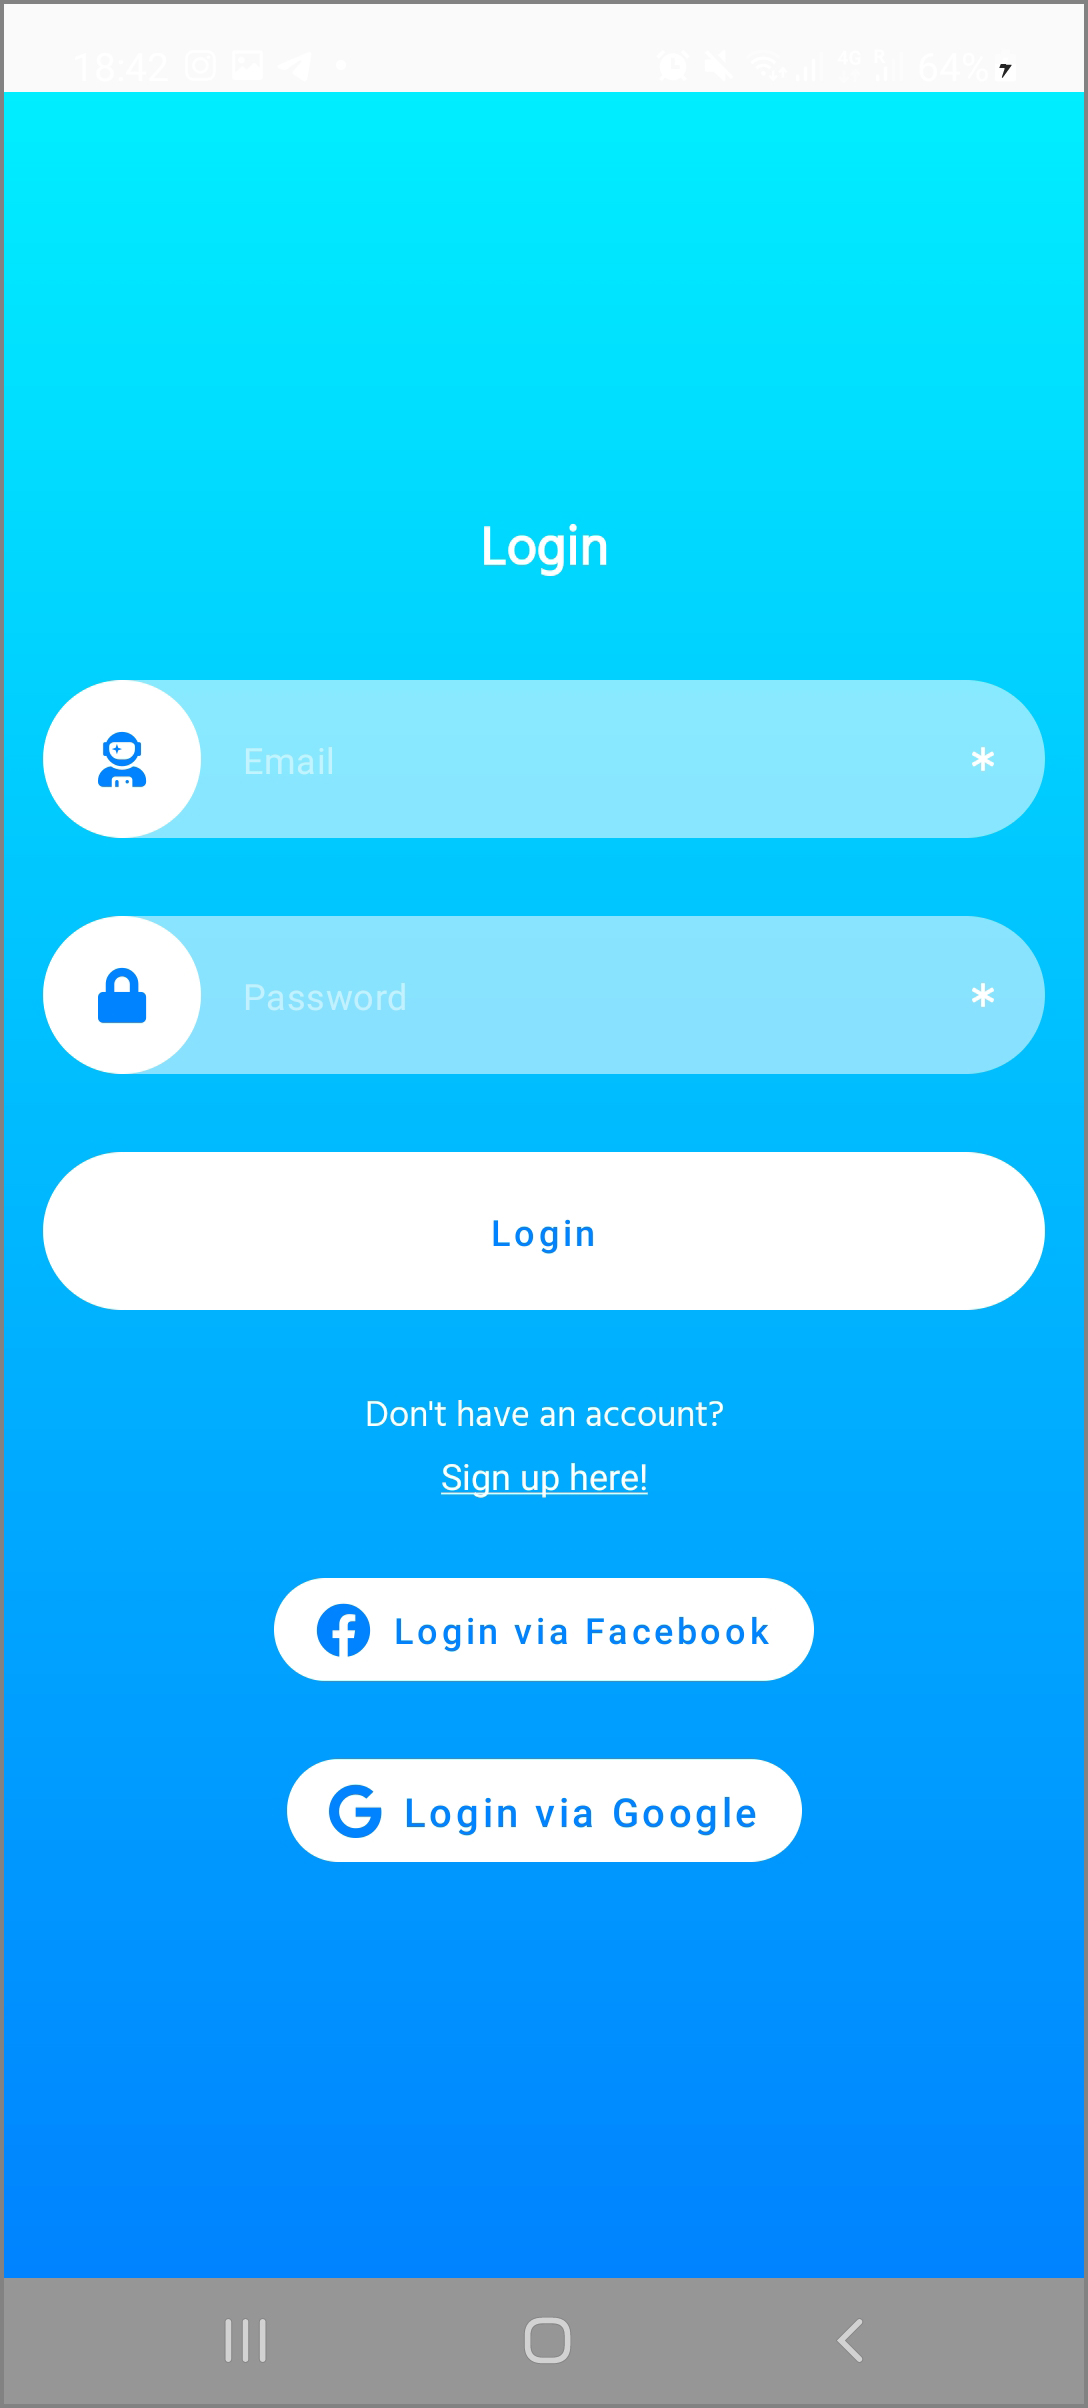
\includegraphics[width=0.5\textwidth]{../Images/UI/Login.jpg}
\caption{\label{fig:dbapiuser}\textbf{Login screen}}
\end{figure} 

Login screen provides users with the option of logging in or registering with email, Google account, or Facebook account. Successfully logging in leads the user to the Main screen of the app.
\newpage

\subsubsection{Main screen}

\begin{figure}[!htb]
\centering
\begin{minipage}{.48\textwidth}
\centering
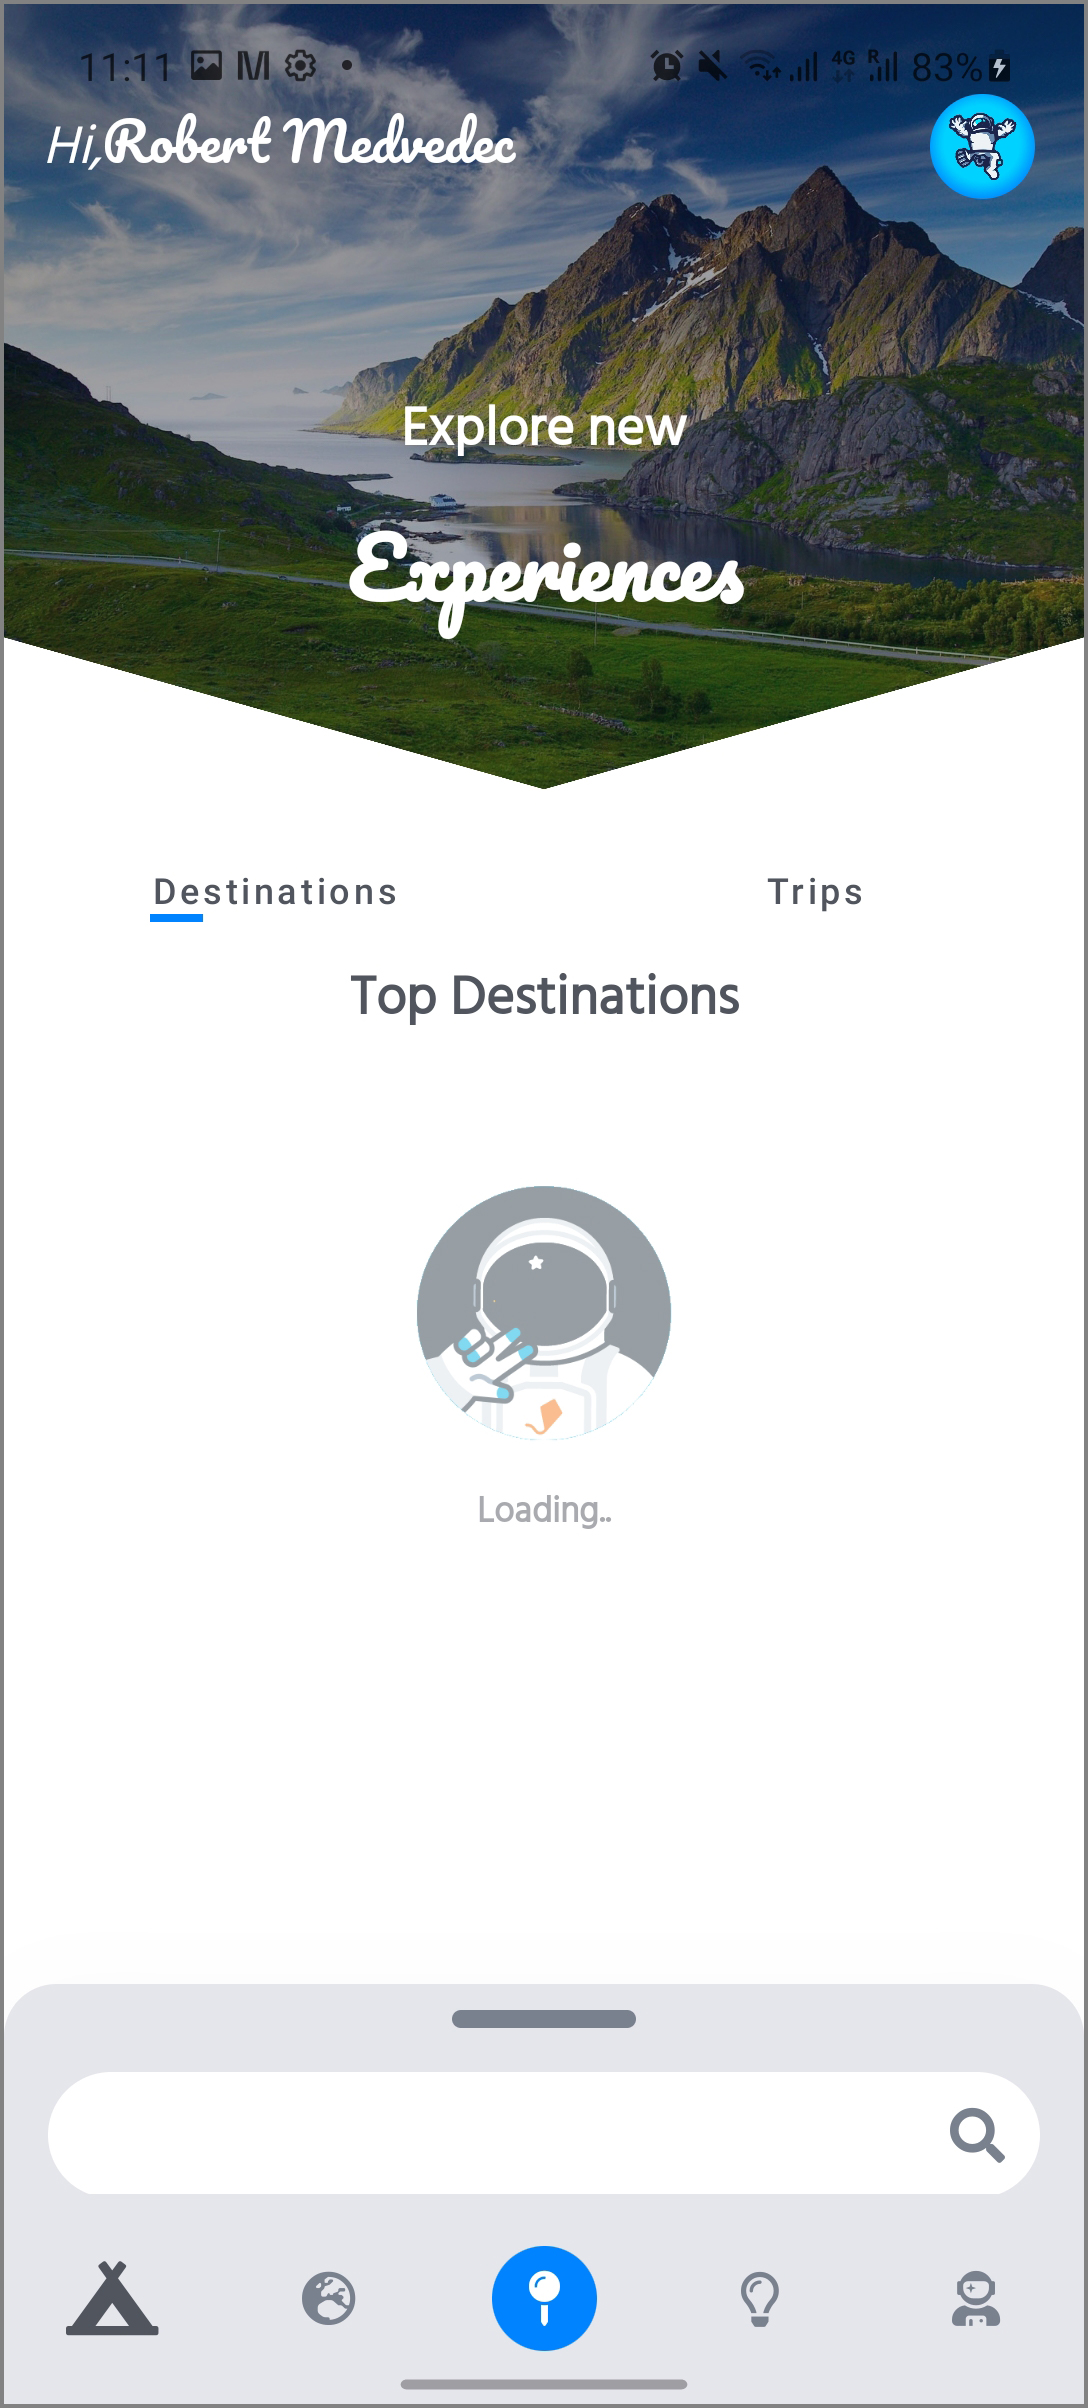
\includegraphics[width=.9\textwidth]{../Images/UI/MainLight.jpg}
\caption{\label{fig:dbapiuser}\textbf{Main screen in light style}}
\end{minipage} 
\begin{minipage}{.48\textwidth}
\centering
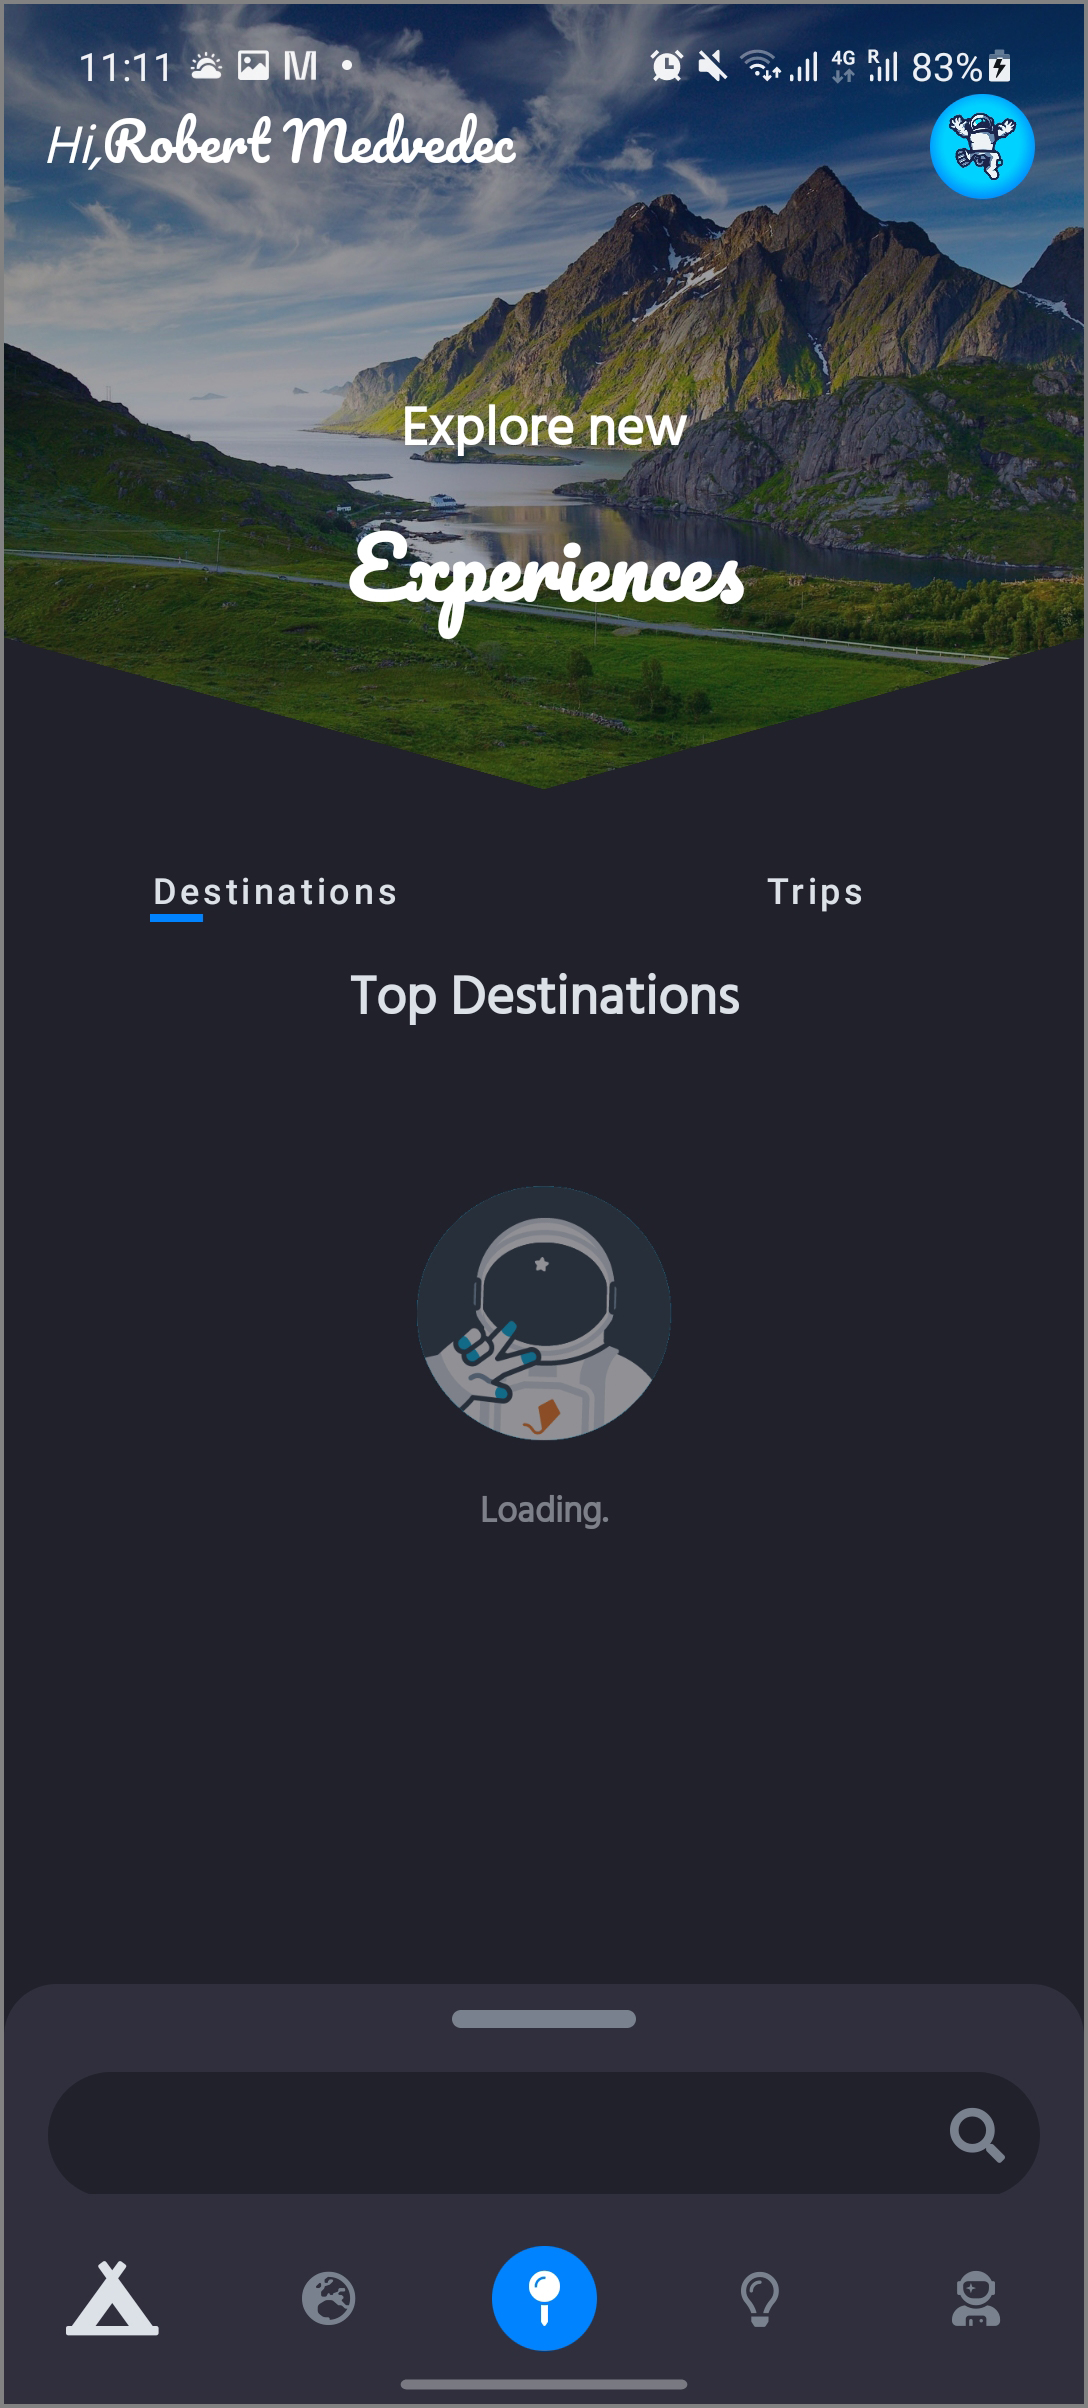
\includegraphics[width=.9\textwidth]{../Images/UI/MainDark.jpg}
\caption{\label{fig:dbapiuser}\textbf{Main screen in dark style}}
\end{minipage}
\end{figure} 

Main screen provides user with the information about the existing destinations and trips. It offers the user a fast way to access some of the information about the locations that they might find useful to build on or to explore.
\newpage
\subsubsection{Map screen}
\begin{figure}[!htb]
\centering
\begin{minipage}{.48\textwidth}
\centering
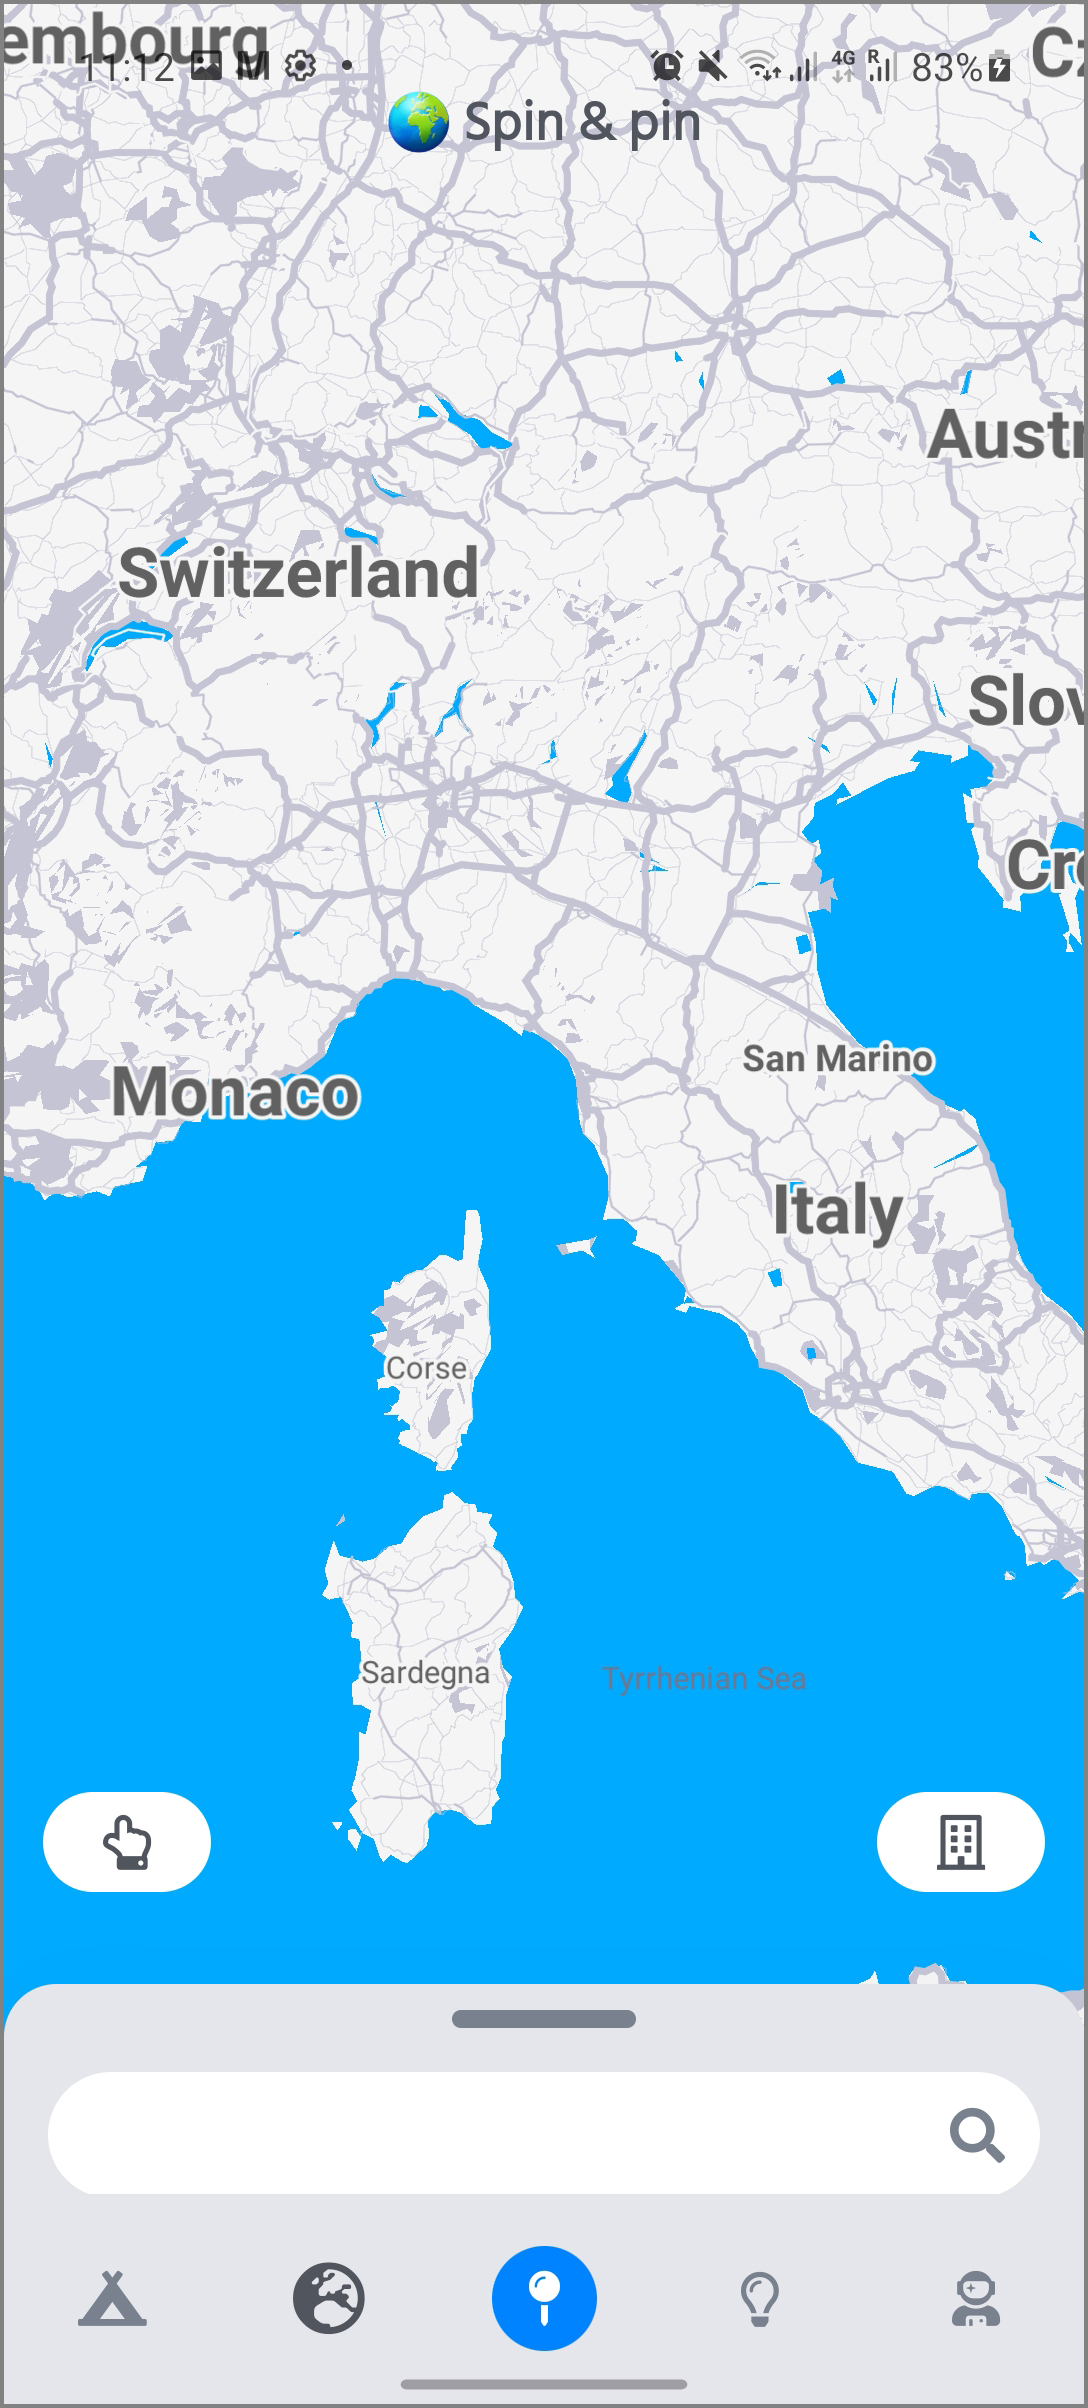
\includegraphics[width=.9\textwidth]{../Images/UI/MapSearchLight.jpg}
\caption{\label{fig:dbapiuser}\textbf{Map screen in light style}}
\end{minipage} 
\begin{minipage}{.48\textwidth}
\centering
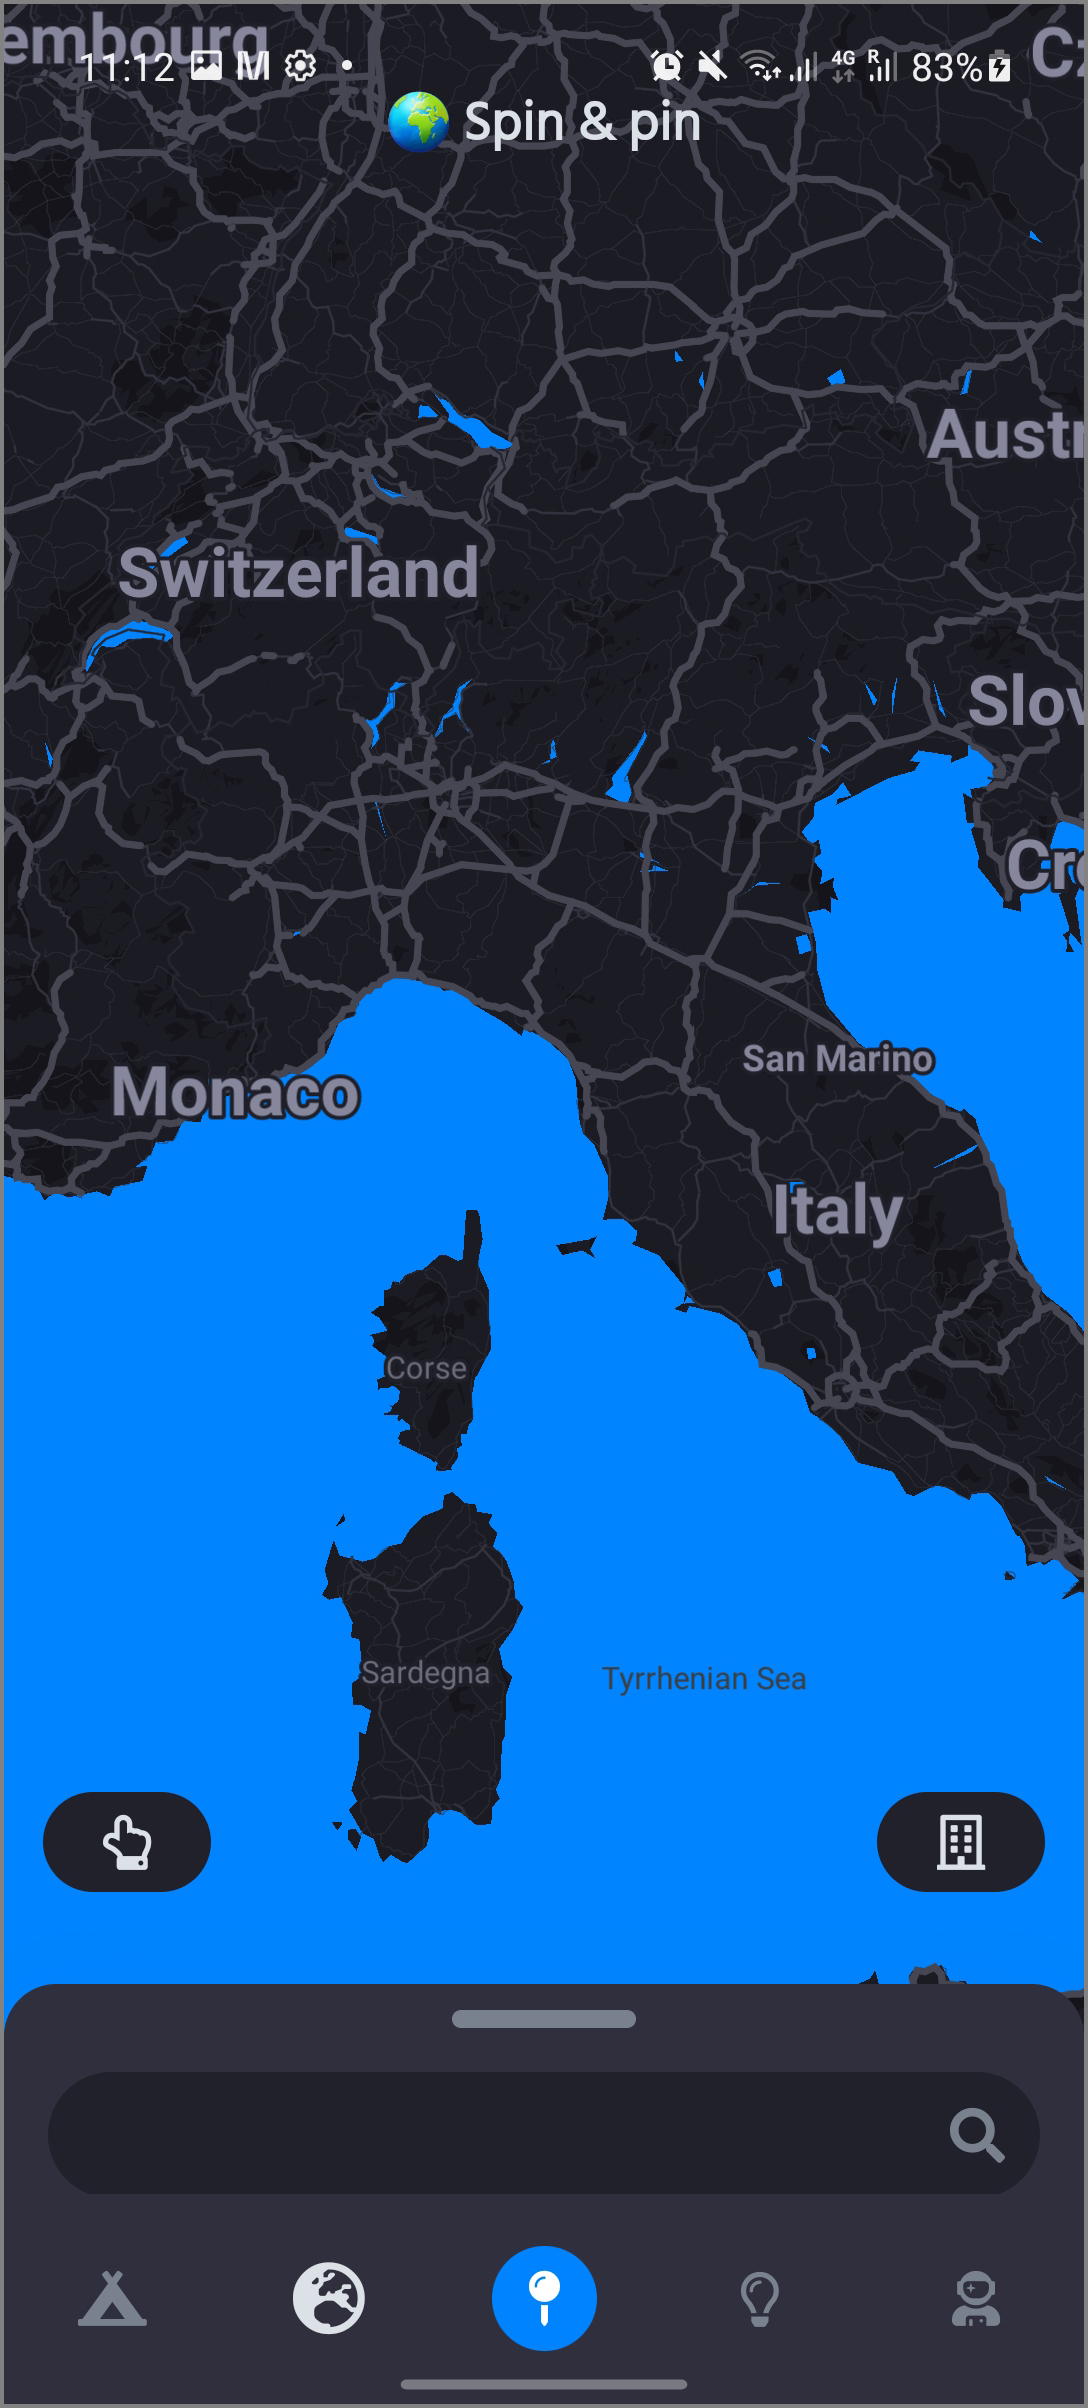
\includegraphics[width=.9\textwidth]{../Images/UI/MapSearchDark.jpg}
\caption{\label{fig:dbapiuser}\textbf{Map screen in dark style}}
\end{minipage}
\end{figure}

Map screen allows users to interactively go through the desired locations on the map and find small icons that represent trips in that area. Map takes into account the boundaries that are shown on the screen and actively adjusts the search parameters, fetching from the database only the trips that are in the current area. Map helps users explore certain areas when they are not sure which specific destination to center their trip around.
\newpage

\subsubsection{Saved trips screen}
\begin{figure}[!htb]
\centering
\begin{minipage}{.48\textwidth}
\centering
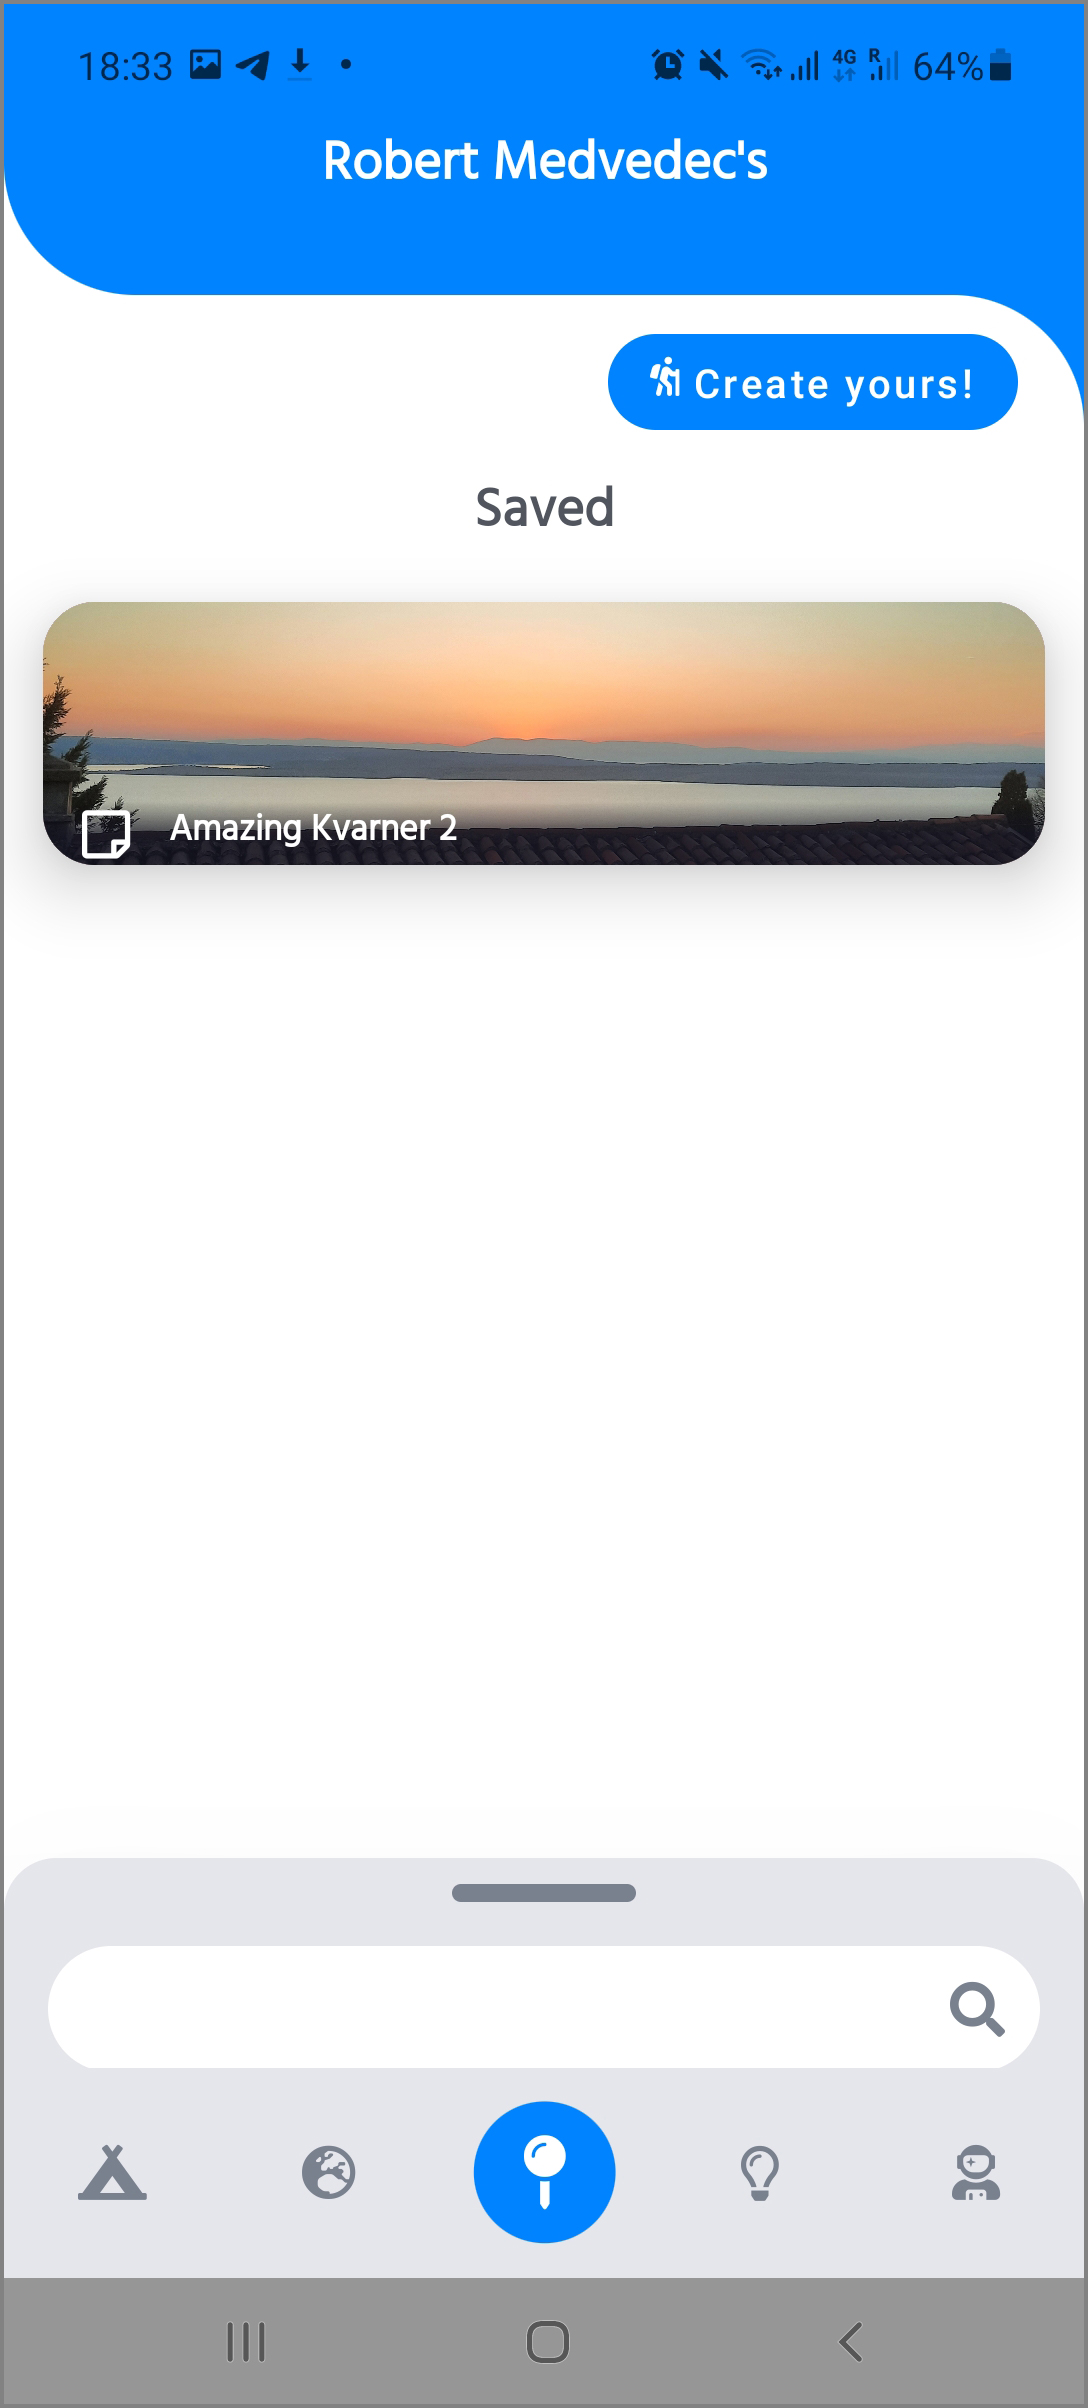
\includegraphics[width=.9\textwidth]{../Images/UI/MyTripsWhite.jpg}
\caption{\label{fig:dbapiuser}\textbf{Saved trips screen in light style}}
\end{minipage} 
\begin{minipage}{.48\textwidth}
\centering
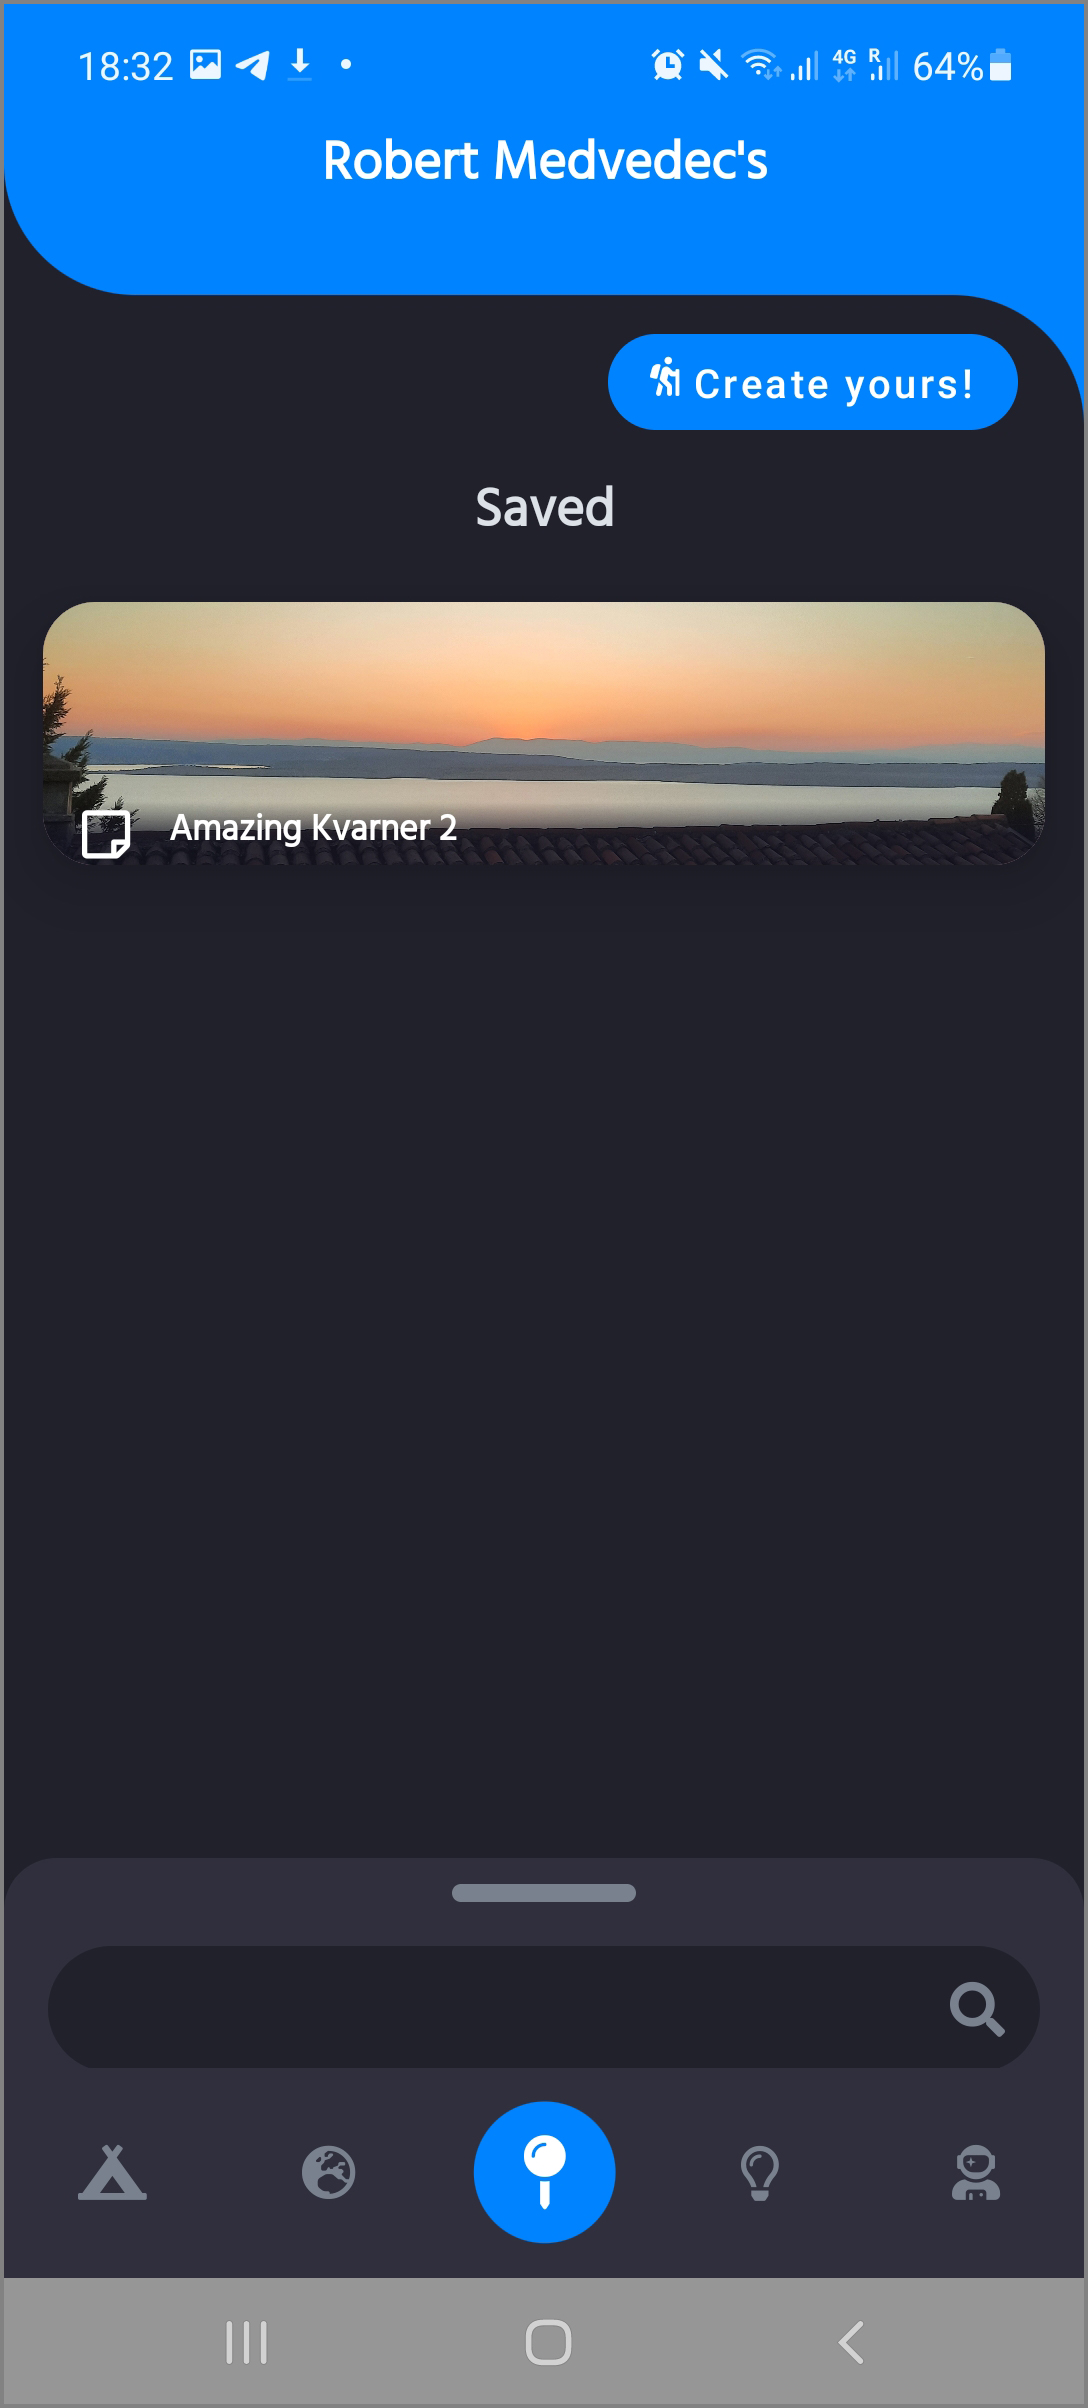
\includegraphics[width=.9\textwidth]{../Images/UI/MyTripsDark.jpg}
\caption{\label{fig:dbapiuser}\textbf{Saved trips screen in dark style}}
\end{minipage}
\end{figure}

Saved trips screen holds the information of all of the trips the user has created or saved. It is also a quick way of finding older trips that users found interesting and allows them to organize their travels in an easy and effective way.
 
\newpage
\subsubsection{Explore screen}
\begin{figure}[!htb]
\centering
\begin{minipage}{.48\textwidth}
\centering
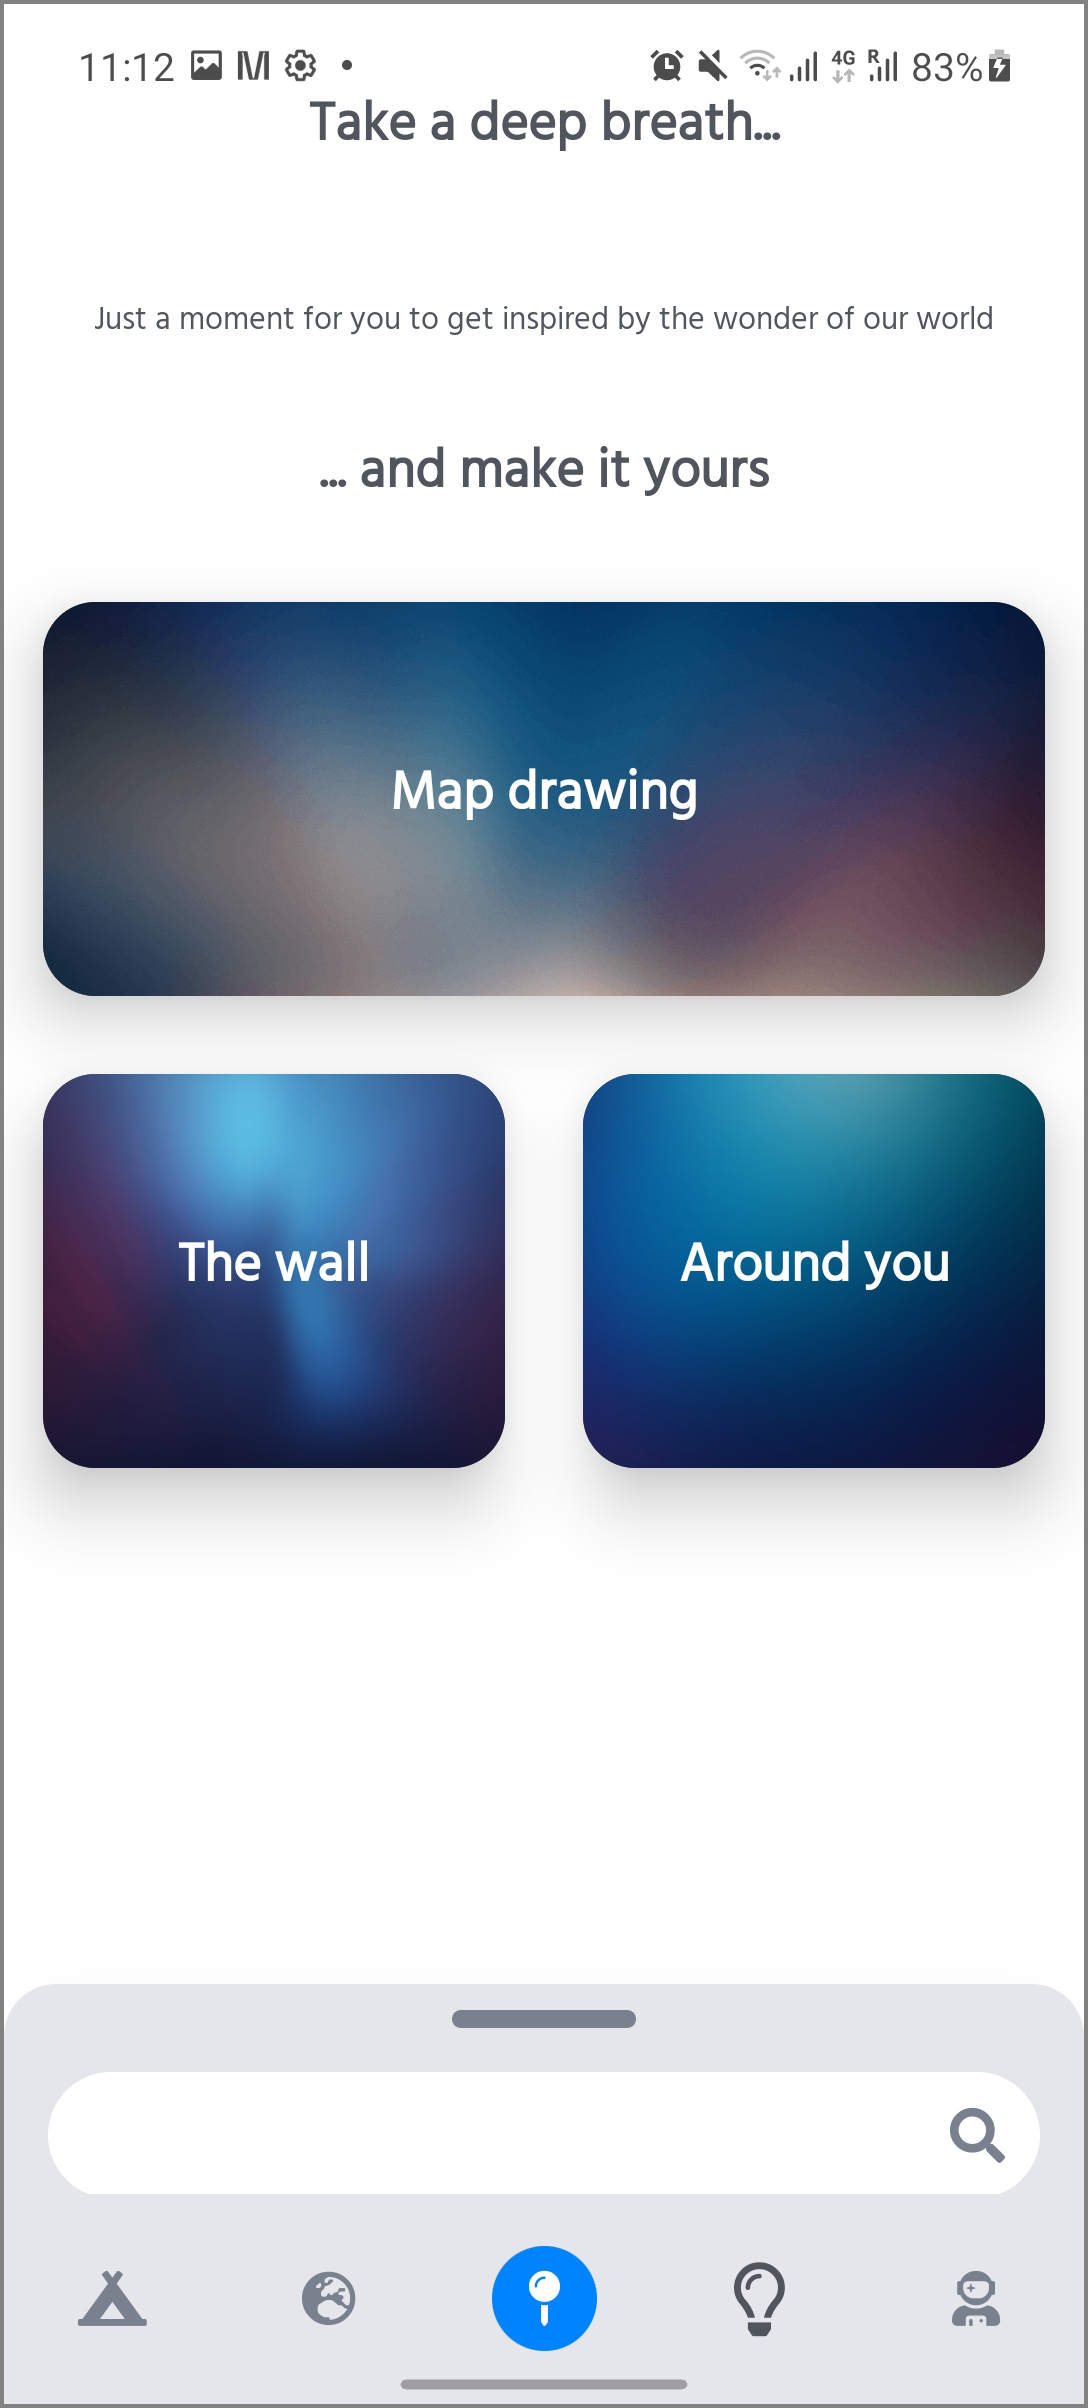
\includegraphics[width=.9\textwidth]{../Images/UI/ExploreLight.jpg}
\caption{\label{fig:dbapiuser}\textbf{Explore screen in light style}}
\end{minipage} 
\begin{minipage}{.48\textwidth}
\centering
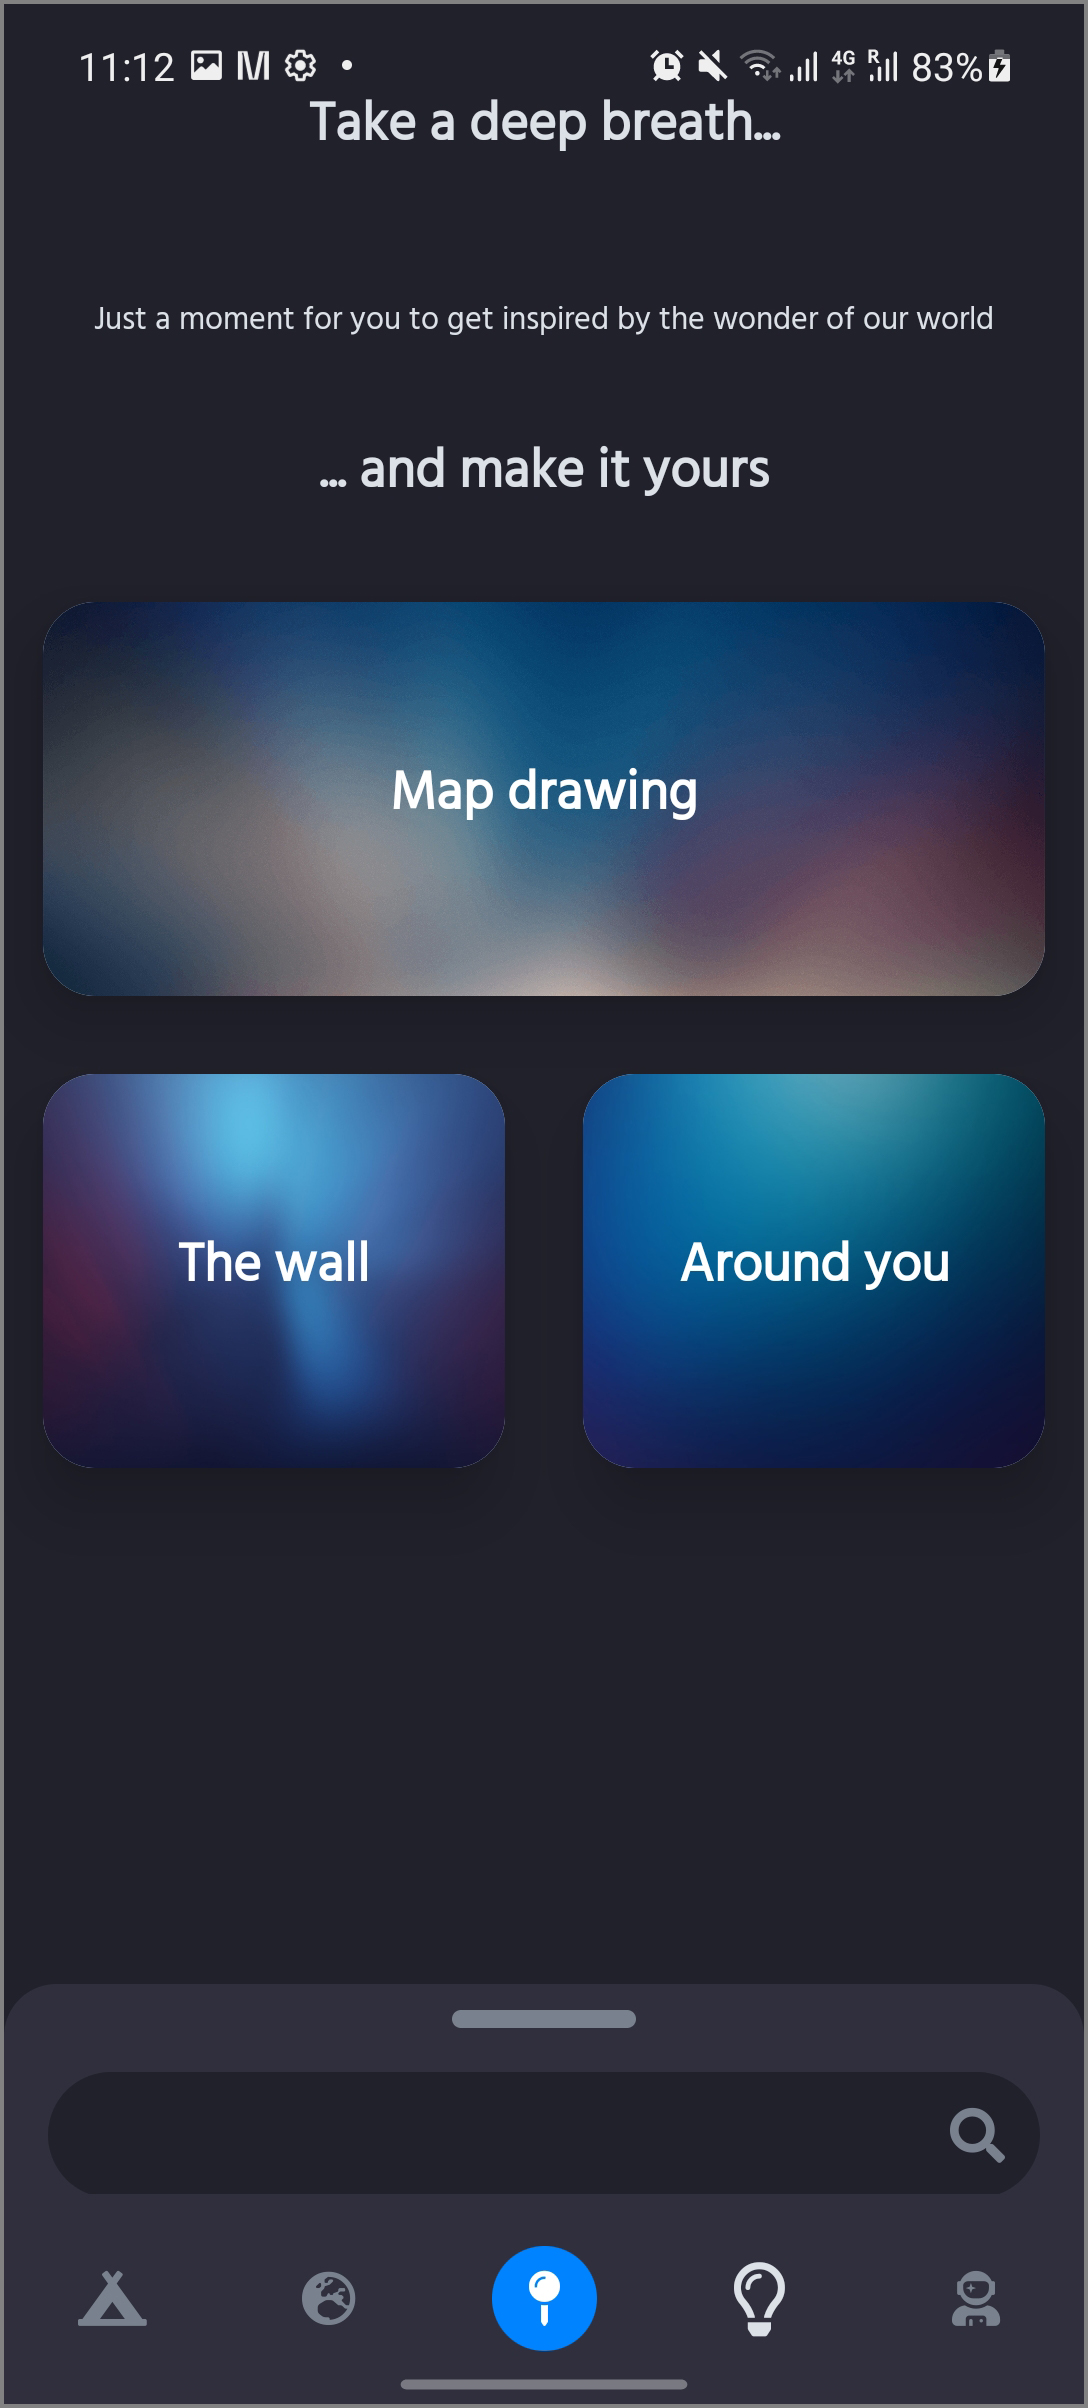
\includegraphics[width=.9\textwidth]{../Images/UI/ExploreDark.jpg}
\caption{\label{fig:dbapiuser}\textbf{Explore screen in dark style}}
\end{minipage}
\end{figure}

Explore screen allows users to search for their future trips in multiple ways. The first way is by searching on the map, and by clicking the 'Map drawing' button, the app takes the user to the previously explained screen.\\ \\
The next option, 'The wall',  - DOESN?T DO ANYTHING NOW. \\ \\
Finally, 'Around you' button asks the user for location permission, and if granted, searches for interesting destinations and trips in the user's vicinity.
 
\newpage
\subsubsection{Settings screen}
\begin{figure}[!htb]
\centering
\begin{minipage}{.48\textwidth}
\centering
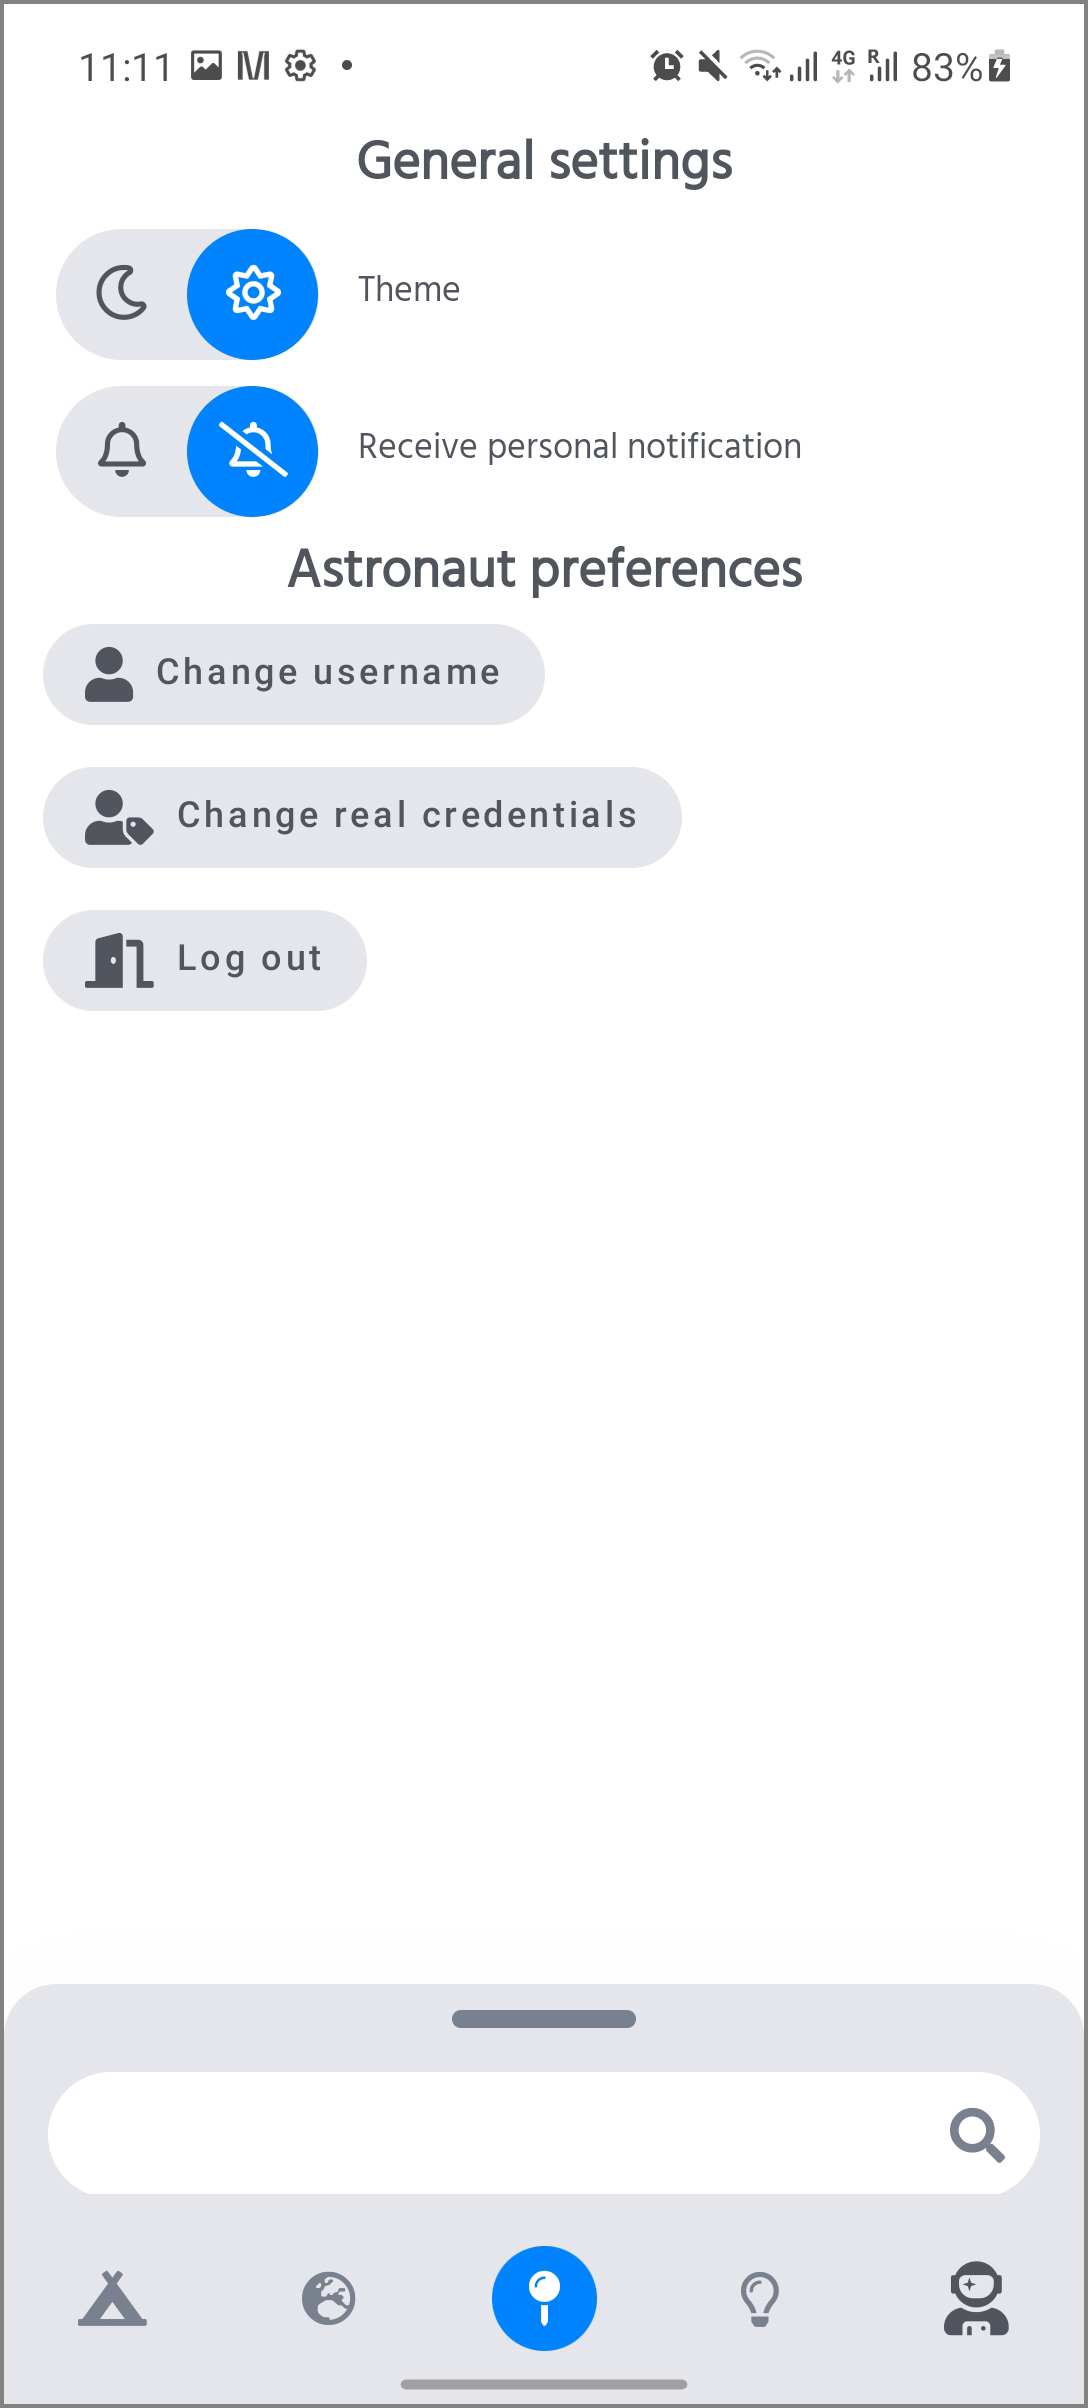
\includegraphics[width=.9\textwidth]{../Images/UI/SettingsLight.jpg}
\caption{\label{fig:dbapiuser}\textbf{Settings screen in light style}}
\end{minipage} 
\begin{minipage}{.48\textwidth}
\centering
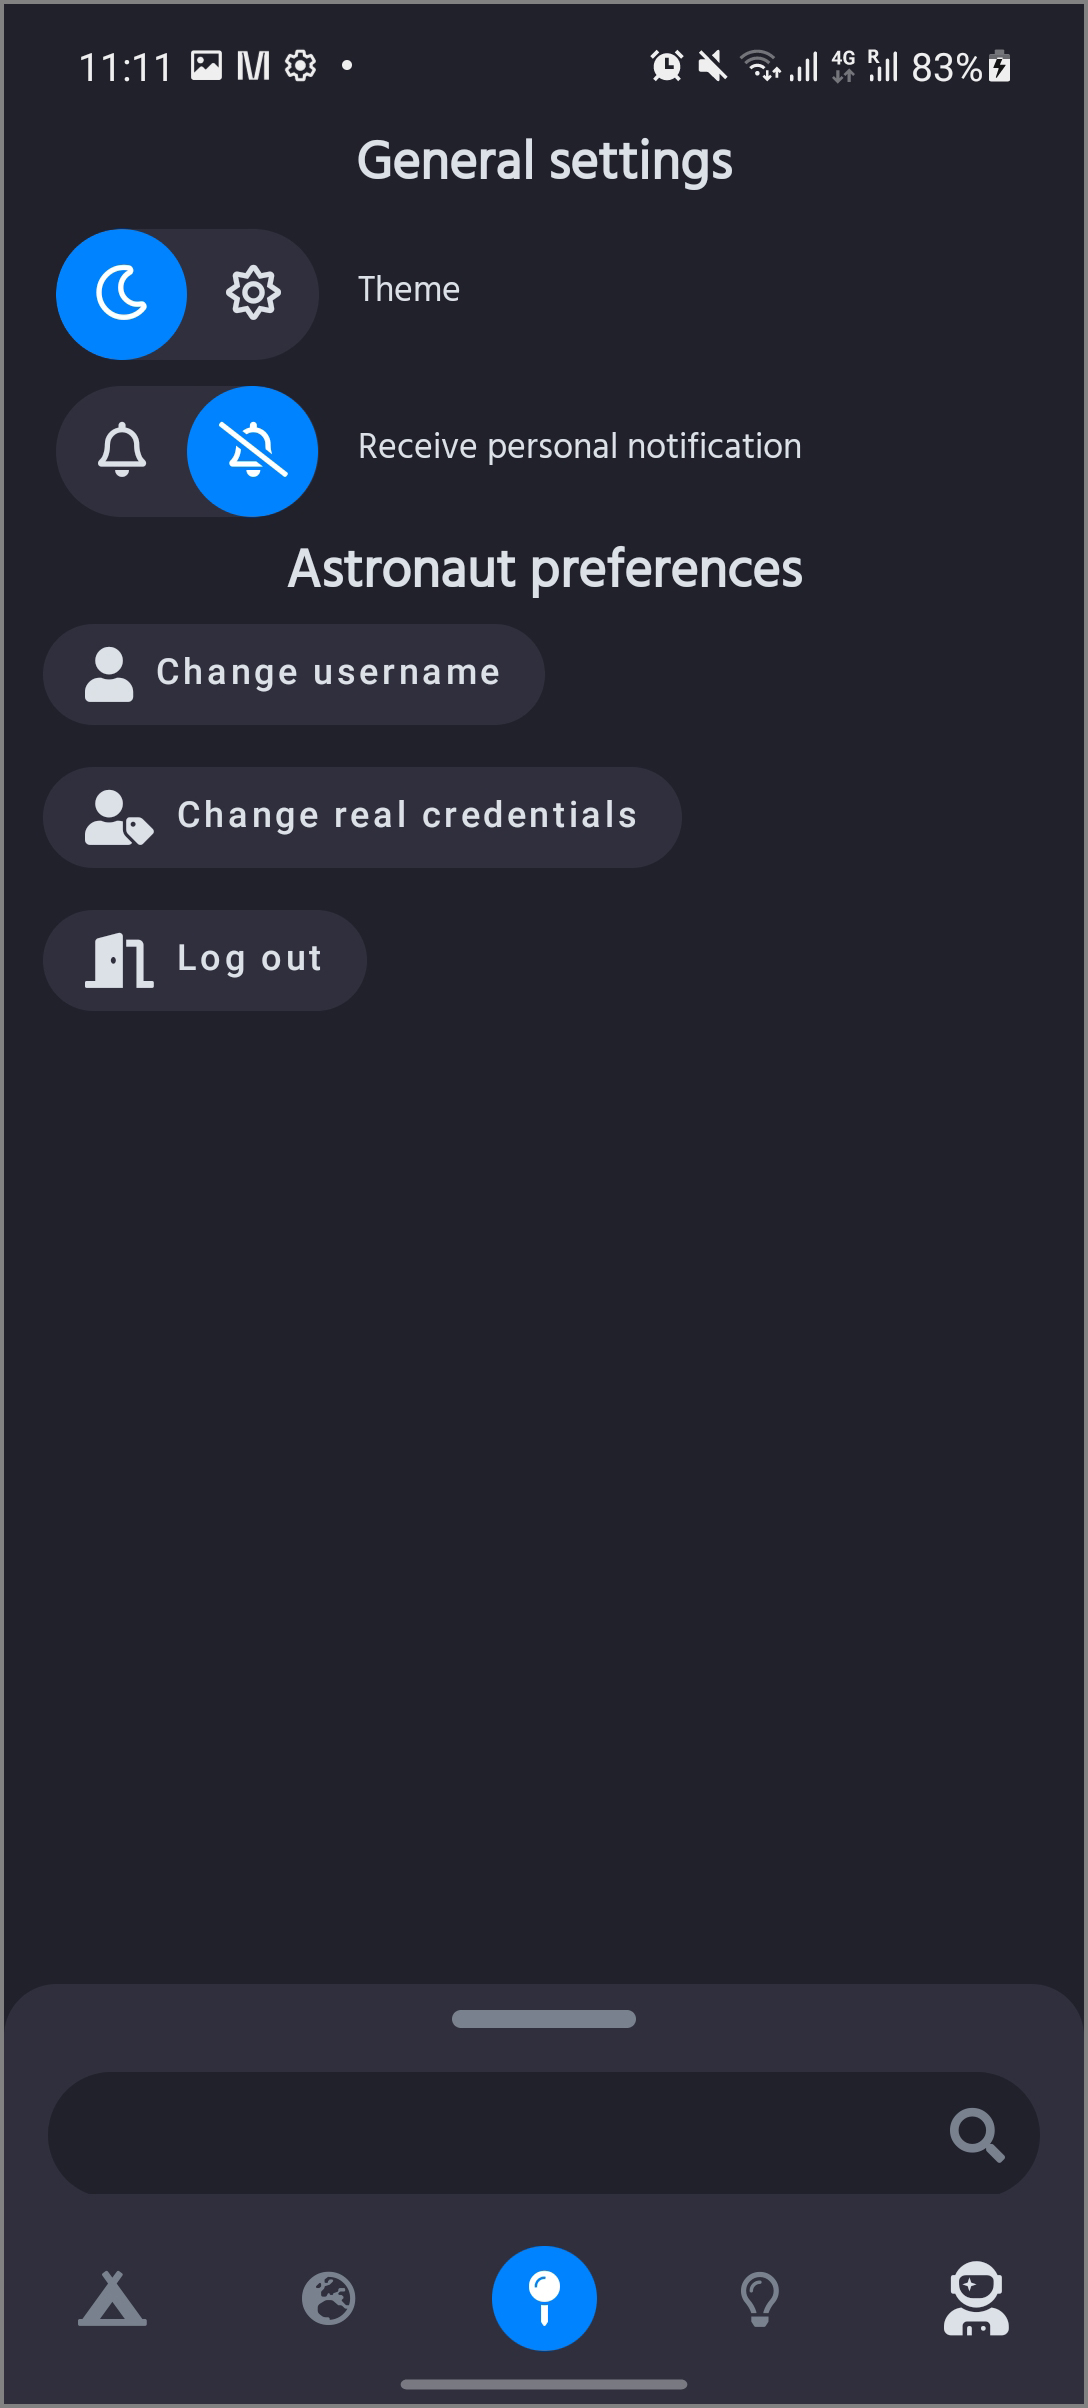
\includegraphics[width=.9\textwidth]{../Images/UI/SettingsDark.jpg}
\caption{\label{fig:dbapiuser}\textbf{Settings screen in dark style}}
\end{minipage}
\end{figure}

Settings screen allows users to change between dark and light theme, to turn the notifications on or off, and to change user preferences such as username and real credentials, which are optional. It also features an option to log out, if user ever wishes to change their account. 
 
\newpage
\subsubsection{Trip creation screen}
\begin{figure}[!htb]
\centering
\begin{minipage}{.48\textwidth}
\centering
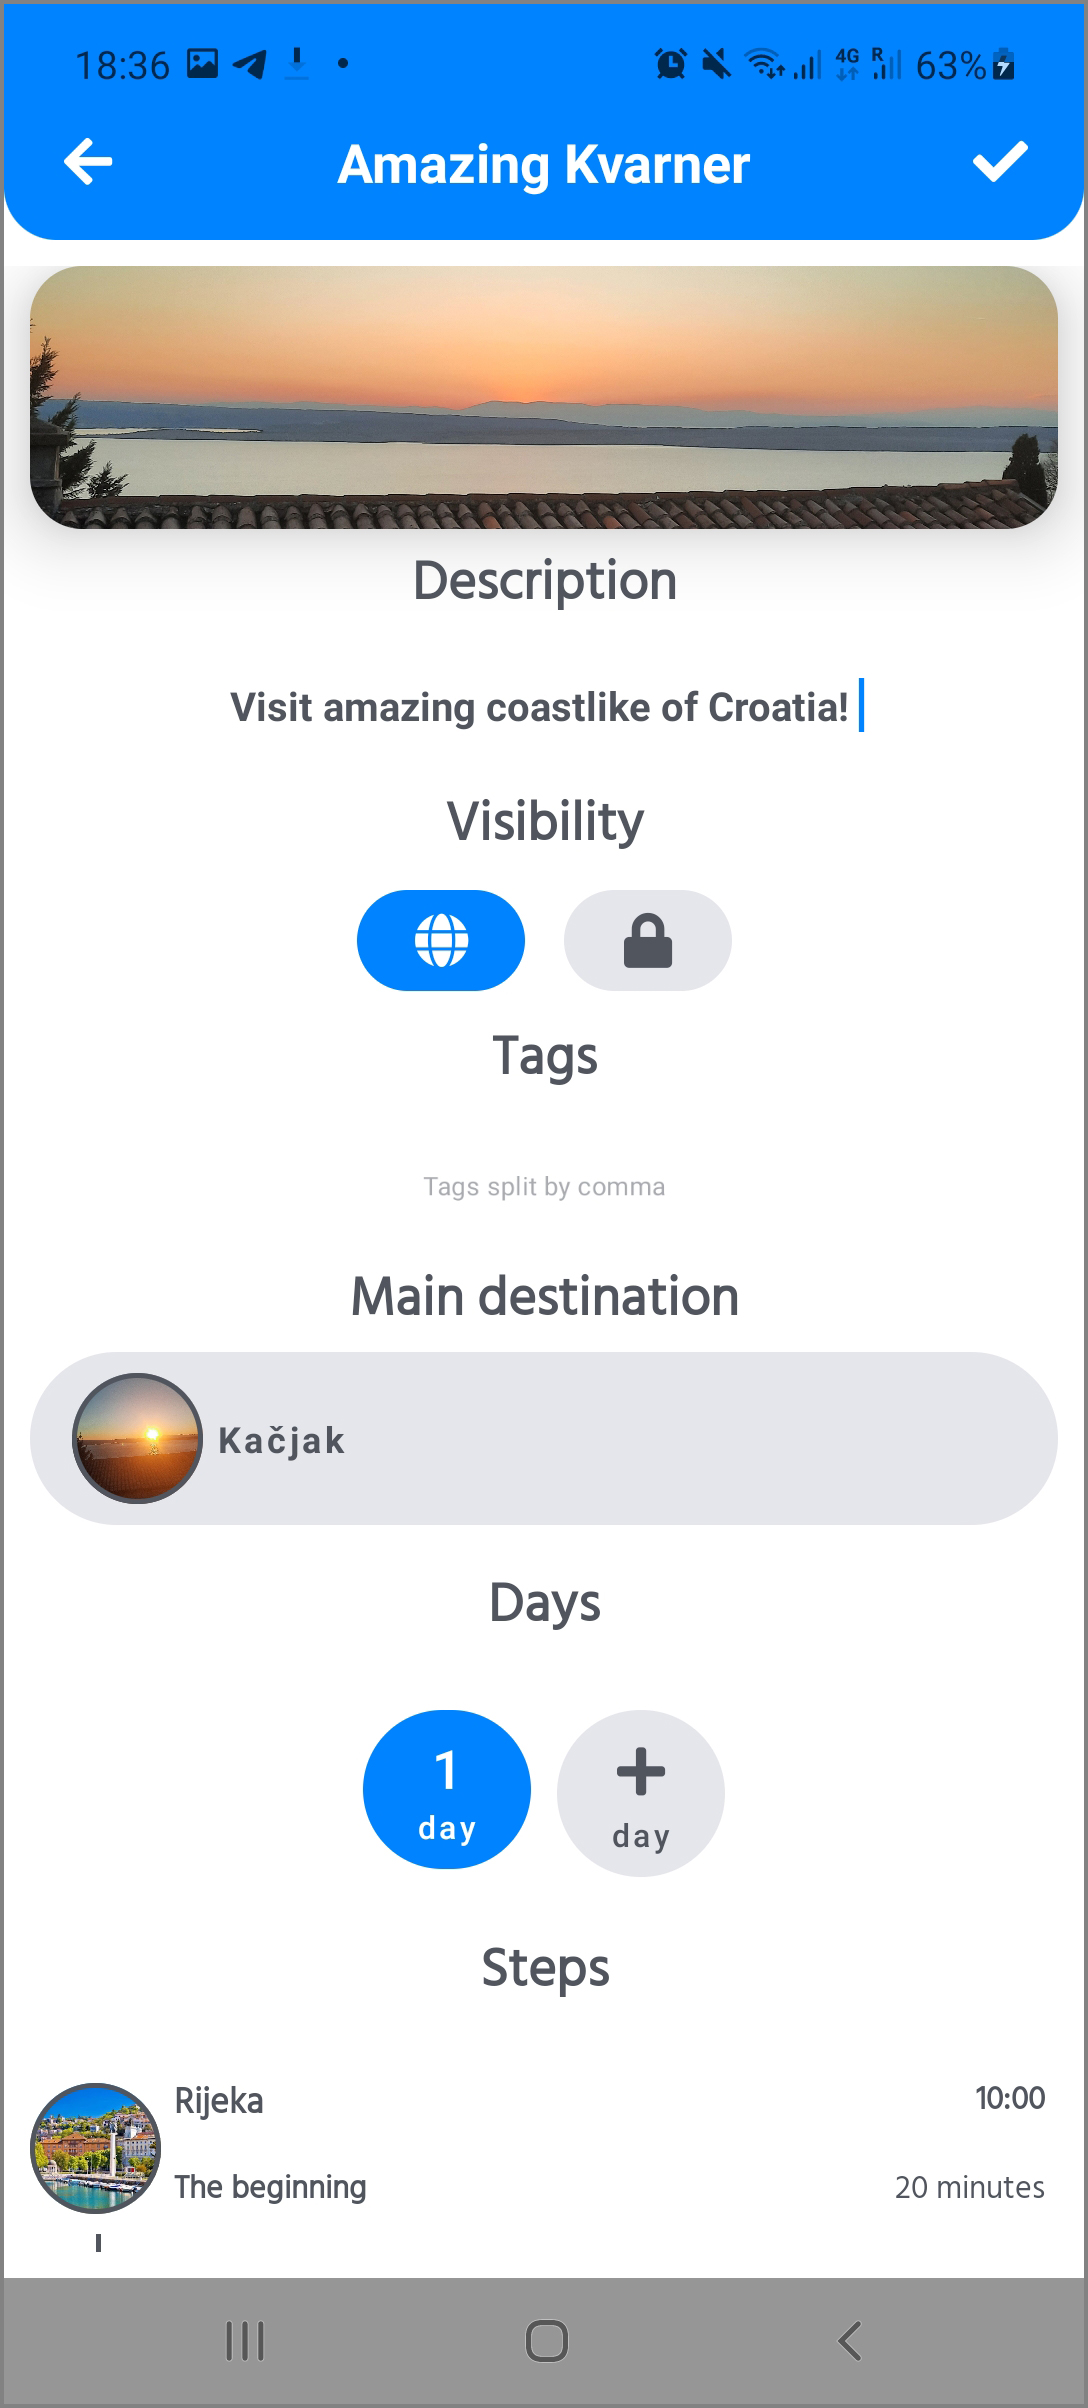
\includegraphics[width=.9\textwidth]{../Images/UI/TripCreateWhite.jpg}
\caption{\label{fig:dbapiuser}\textbf{Trip creation screen in light style}}
\end{minipage} 
\begin{minipage}{.48\textwidth}
\centering
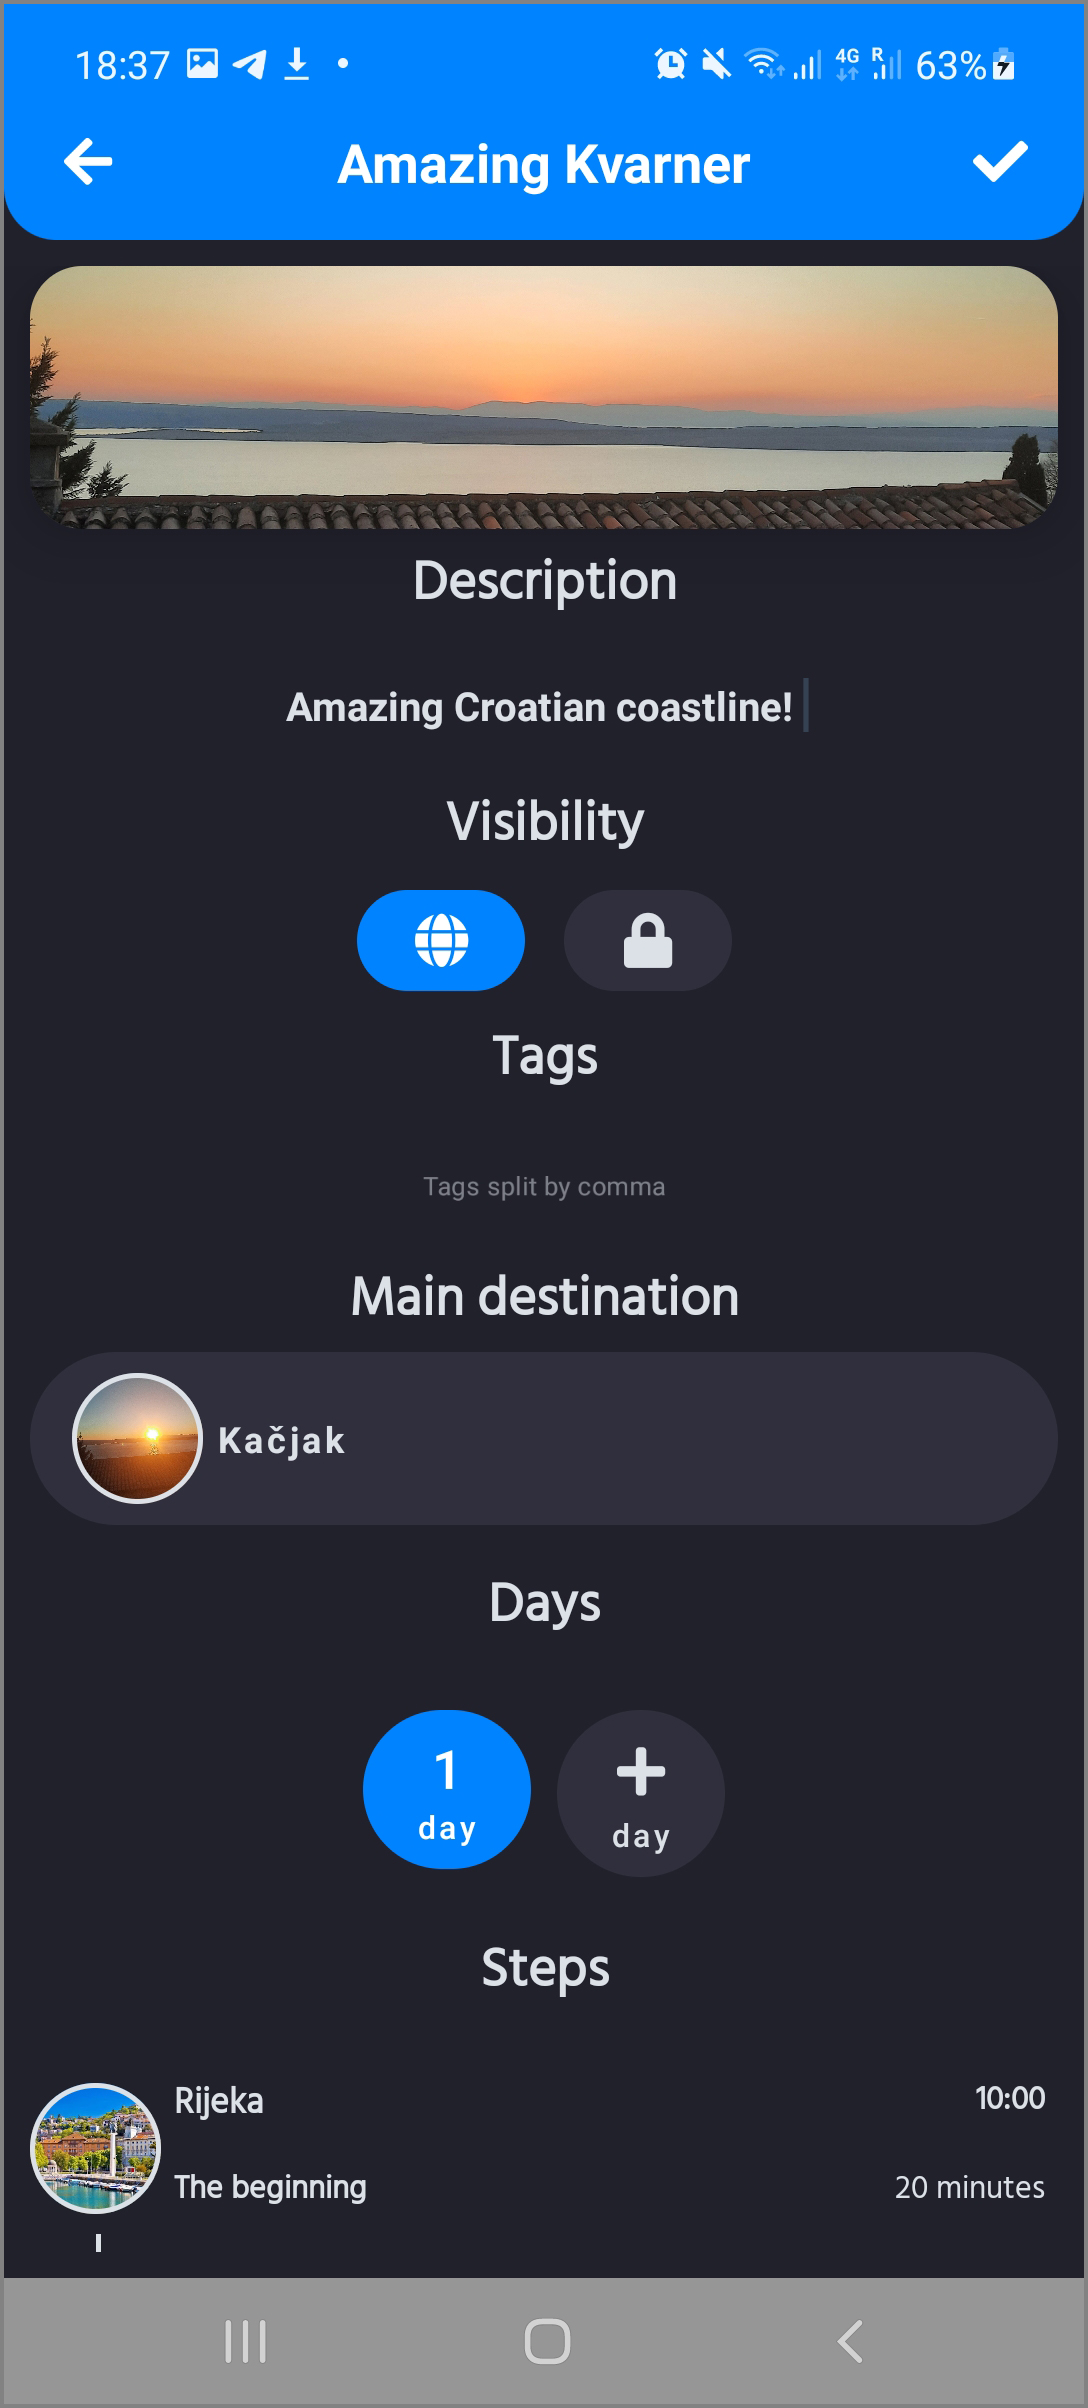
\includegraphics[width=.9\textwidth]{../Images/UI/TripCreateDark.jpg}
\caption{\label{fig:dbapiuser}\textbf{Trip creation screen in dark style}}
\end{minipage}
\end{figure}

This is the way the trip creation looks like, with its functionality previously explained in the document. This screen also features several sub screens, which are not presented in the document due to conciseness.